\chapter{Funções}\label{cap:Functions}

\epigraph{``O ego é o pior inimigo do Eu, mas o Eu é o melhor amigo do ego... O ego é um péssimo senhor, mas é um ótimo servidor''.}{Bhagavad Gita}

\section{Conceitos, Definições e Nomenclaturas}\label{sec:FunctionsDefinitions}

Após o conceito importantíssimo de conjunto, o componente mais importante na matemática é provavelmente a noção de função. O autor deste documento não hesita em afirmar que você, leitor, com certeza já teve contato com a ideia de função, seja em seus cursos de nível primário, secundário ou mesmo mais recentemente em seus cursos de cálculo diferencial e integral, estatística ou cursos de física.

Dado este encontro anterior do leitor sobre o assunto, o autor fica confortável em pedir que o leitor faça uma pequena pausa e tente lembrar de seus cursos anteriores e responda para si ao questionamento: \textbf{o que é uma função}?

Bem, para muitos físicos, estatísticos e alguns matemáticos (não todos\footnote{Um visão interessante é aquela apontada em \cite{levin2021}, que descreve uma função como sendo um objeto com quatro descrições simultâneas: uma algébrica, uma numérica, uma gráfica e uma descritiva (ou em palavras).}), uma função é vista meramente como sendo um mapeamento (ou transformação) entre os elementos de dois conjuntos \cite{abe1991-TC}. Por outro lado, em obras tais como \cite{sussana2010-MD, lipschutz1971-Topo, lipschutz1978-TC, lipschutz2013-MD, Gerard2021discreta} uma função é vista como uma caso particular de relação entre dois conjuntos, ou seja, em última análise para esse grupo de pessoas uma função é exatamente um conjunto\footnote{Para melhor entender essa visão talvez o leitor deva revistar os Capítulos \ref{cap:Sets} e \ref{cap:Relations} e revisar as definições apresentadas nos mesmo.}. Já em \cite{edward2019-MD, fmcbook} é apresentado uma visão mais mecanicista da ideia de função, essa visão captura a ideia de função enquanto uma máquina\footnote{Para cientistas da computação os termos máquina e programa são sinônimos.} (ou caixa preta) que transforma as entradas (\textit{inputs}) em saídas (\textit{outputs}), essa visão é ilustrada pela Figura \ref{fig:FuncaoBlackBox}. 

\begin{figure}[h]
	\centering
	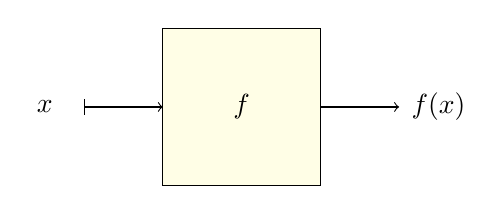
\begin{tikzpicture}
		\draw [rounded corners=0mm, fill=yellow!10]  (-1,1)--(-1,-1)--(1,-1)--(1,1)--cycle;
		\draw[->]  (1.0,0) -- (2.0,0.0);
		\draw[|->]  (-2.0,0) -- (-1.0,0.0);
		\node (f) at (0,0) {$f$};
		\node (fx) at (2.5,0) {$f(x)$};
		\node (x) at (-2.5,0) {$x$};
	\end{tikzpicture}
	\caption{Visão de uma função de uma variável enquanto uma máquina (ou caixa preta).}
	\label{fig:FuncaoBlackBox}
\end{figure}

Há também a ideia de função como uma estrutura \cite{judith2021}, com componentes bem estabelecidos. Essa visão é capaz (como será mostrado a seguir) de capturar todas as outras ideias de função.  Neste documento, a formalização da ideia de função como uma estrutura será apresentada gradualmente, trançando paralelos com as linguagens de programação que possuam um sistema de tipos. Isso será adotado para tornar o texto mais didático e interessante ao leitor de computação, além disso, irá aproximar os tópicos teóricos (as funções) dos tópicos práticos (os programas). Entretanto, essa forma de apresentação não será menos rigorosa que outras fontes bibliográficas. O objetivo deste texto é apresentar da forma mais precisa e detalhada a noção de função, tanto do ponto de vista puramente formal, como do ponto de vista prático (da construção de algoritmos).

Este documento inicia o estudo sobre funções apresentando ao leitor a ideia básica de assinatura de função, isto é, a seguir será apresentado a representação sintática (ou de tipagem) que descreve as funções, ou seja, o componente descritivo como mencionado em \cite{levin2021}.

\begin{definicao}[Assinatura de Função]\label{def:AssinaturaFuncao}
	Sejam $A$ e $B$ dois conjuntos a assinatura da função de $A$ em $B$ nomeada como $f$ corresponde a uma palavra da forma $f: A \rightarrow B$.
\end{definicao}

A Definição \ref{def:AssinaturaFuncao} permite facilmente deduzir que em qualquer função existem três elementos básicos, sendo eles: um nome (rótulo ou símbolo funcional), um conjunto de partida e um conjunto de chegada. Por convenção, o nome de uma função deve ser sempre iniciado por caracteres latinos, no caso de usar índices apenas o último caractere do nome deve ser indexado.

\begin{exemplo}\label{exe:AssinaturaFuncao}
	São exemplos de assinaturas de funções:
	\begin{itemize}
		\item[(a)] $g : \mathbb{N} \rightarrow \mathbb{Z}$.
		\item[(b)] $sqrt : \mathbb{R} \rightarrow \mathbb{R}$.
		\item[(c)] $k_1 : A \times B \rightarrow \mathbb{C}$.
		\item[(d)] $loc_2 : D \rightarrow \mathbb{R} \times \{0,1\}$.
		\item[(e)] $min : \mathbb{R}^n \rightarrow \mathbb{R}$.
		\item[(f)] $BUSCA : \mathbb{Z}^n \times \mathbb{Z} \rightarrow \{0,1\}$.
		\item[(g)] $BUSCA : \mathbb{R}^n \times \mathbb{R} \rightarrow \{0,1\}$.
    \item[(h)] $mydouble: \mathbb{Z} \rightarrow \mathbb{Z}$.
	\end{itemize}
\end{exemplo}

\begin{cuidado}
  {\color{red}Tenha MUITO cuidado}, apesar das assinaturas nos itens (f) e (g) do Exemplo \ref{exe:AssinaturaFuncao} terem o mesmo nome, elas não são iguais, pois diferem no conjunto de partida, e assim não são a mesma assinatura. Esse tipo de cenário recebe o nome de sobrecarga\footnote{Na literatura sobre linguagens de programação é usado o termo \textit{override}.}, isto é, o símbolo funcional $BUSCA$ está sobrecarregado para identificar duas funções distintas.
\end{cuidado}

Diversas linguagens de programação tais como C, C++, Haskell e Java (entre outras) apresentam a possibilidade de definir assinaturas de funções. Na linguagem C, por exemplo, as assinaturas de funções que compõem uma biblioteca são geralmente reunidas em um arquivo de \textit{header}, isto é, um arquivo com a extensão ``.h'', para mais detalhes consulte \cite{paulo2009algoritmos}, a seguir é exemplificado um arquivo de \textit{header}.

\begin{figure}[h]
	\lstinputlisting[style=Cstyle]{codes/assinatura.h}
	\caption{Exemplo de um arquivo .h contendo assinaturas na linguagem C.}
	\label{fig:AssinaturasEmC}
\end{figure}

\begin{figure}[h]
	\lstinputlisting[style=Hstyle]{codes/assinatura.hs}
	\caption{Exemplo de um arquivo com assinaturas na linguagem Haskell.}
	\label{fig:AssinaturasEmHaskell}
\end{figure}

%\begin{nota}[Sobre programação versus matemática!]
%  Considere a assinatura no item (h) do Exemplo \ref{exe:AssinaturaFuncao}, ou seja, a assinatura da função de inteiros em inteiros nomeado como $mydouble$.
%\end{nota}

Um conceito indiretamente esboçado pela ideia de assinatura de função, é o de tipagem da função, sempre que a assinatura é da forma $f: A \rightarrow B$ pode-se dizer que $f$ é uma função do tipo ``$A$ em $B$'', ou mesmo que ``$f$ é um tipo seta de $A$ para $B$'', a noção de ``tipo seta'' é uma nomenclatura indiretamente ligado a ideia de teoria dos tipos.

%\begin{nota}\label{note:TipoFuncao}
%	Durante os anos o autor encontrou programadores focados em linguagens imperativas que erravam a seguinte questão: ``Qual é o tipo da função reverse (definida na linha 2 da Figura \ref{fig:AssinaturasEmC})?'' Eles em geral respondiam que a função é do tipo int quando na verdade é do tipo seta de int em int, ou seja, sua assinatura seria da forma, reverse: int $\rightarrow$ int.
%\end{nota}

Como dito anteriormente uma função pode ser vista como uma máquina que transforma entradas em saídas, mas note que para que isso aconteça a máquina deve de alguma forma realizar ações sobre a entrada, ou seja, a máquina deve ``operar'' sobre a entrada. Esse conceito de como a máquina deve operar sobre as entradas é descrito por uma propriedade $P$ que define uma relação de mapeamento\footnote{Alguns textos usam a nomenclatura lei de formação, ver por exemplo \cite{carmo2013}.}

\begin{definicao}[Relação de mapeamento]\label{def:RelacaoMapeamento}
	Dado dois conjuntos $A$ e $B$ e seja $x \in A$ e $y \in B$ a relação de mapeamento definida por uma propriedade $P$ corresponde  ao seguinte conjunto 
	$$\varepsilon = \{(x, y)\mid P\}$$ 
  tal que a propriedade $P$ deve satisfazer a seguinte condição: se os pares $(x, y_1),$ $(x, y_2)$ satisfazem $P$, então obrigatoriamente $y_1 = y_2$.
\end{definicao}

Note que a Definição \ref{def:RelacaoMapeamento} apenas descreve que para cada entrada (variável) $x$ existirá uma única saída $y$ tal que $x$ e  $y$ estão relacionados por uma certa propriedade $P$.

\begin{exemplo}\label{exe:RelacaoConstrucao}
	São exemplos de relações de mapeamento:
	\begin{itemize}
		\item[(a)] $\{(x, y) \in \mathbb{R}^2 \mid y = \log_2(x + 1)\}\}$
		\item[(b)] $\{(w_1w_2w_3\cdots w_m, y) \in E^2 \mid y = w_3\cdots w_mw_1w_2\}$ onde $E$ é o conjunto de todas as palavras do português com três letras ou mais e $w_i$ representa o $i$-ésimo símbolo de uma palavra $w$.
		\item[(c)] $\{(x, y) \in \mathbb{N}^2 \mid y = 14\}$.
		\item[(d)] $\Big\{(x_1, x_2, x_3, y) \in \mathbb{R} \times \mathbb{R} \times \mathbb{R}^*_+ \times \mathbb{R} \mid y = \sqrt[x_3]{\displaystyle\frac{1}{2}x_1 + x_2}\Big\}$.
	\end{itemize}
	Não são exemplos de relações de mapeamento:
	\begin{itemize}
		\item[(e)] $\{(x, y) \in N_P \times I_P\}$ onde $N_P$ é o conjunto de todos os nomes de pessoas e $I_P$ é o conjunto de naturais que representam idades, note que em tal relação é permitido que $(\text{Fátima}, 10), (\text{Fátima}, 55)$ estejam nesse conjunto, portanto, esse conjunto não satisfaz a Definição \ref{def:RelacaoMapeamento}.
		\item[(f)] $\{(x, y) \in \mathbb{R}  \mid x = y^2\}$, note que $(25, 5)$ e $(25, -5)$ pertence a tal conjunto e, portanto, esse conjunto não satisfaz a Definição \ref{def:RelacaoMapeamento}.
	\end{itemize}
\end{exemplo}

\begin{nota}
  No item (c) do Exemplo \ref{exe:RelacaoConstrucao} descreve que para qualquer $x$ o $y = 14$, ou seja, para todo $x$ tem-se que o par $(x, 14)$ está na relação. Esse tipo de relação de mapeamento será aqui chamada de \textbf{relação de mapeamento constante}. 
\end{nota}

Agora que foram apresentados estes conceitos fundamentais pode-se continuar o desenvolvimento deste texto com a formalização da ideia de função.

\begin{definicao}[Função]\label{def:Funcao}
	Dado uma assinatura $f: A \rightarrow B$ e seja $\varepsilon \subseteq A \times B$ uma relação de mapeamento, a estrutura $\langle f: A \rightarrow B, \varepsilon \rangle$ é uma função.
\end{definicao}

\begin{exemplo}\label{exe:Funcoes}
	São exemplos de funções:
	\begin{itemize}
		\item[(a)] $\langle dob: \mathbb{N} \rightarrow  \mathbb{N},  \{(x, y) \in \mathbb{N}^2 \mid  y = 2x\} \rangle$.
		\item[(b)] $\langle mul: \mathbb{R} \times \mathbb{R} \rightarrow  \mathbb{N},  \{((x, y), z) \in \mathbb{R}^2 \times \mathbb{R} \mid  z = xy\} \rangle$.
		\item[(c)] $\langle sqroot: \mathbb{N} \rightarrow \mathbb{N},  \{(x, y) \in \mathbb{N}^2 \mid  y^2 = x\} \rangle$.
		\item[(d)] $\langle one: \mathbb{Z}^2 \rightarrow  \{1\},  \{((x, y), 1) \in \mathbb{Z}^2 \times \{1\} \mid  1 = x+y\} \rangle$.
		\item[(e)] $\langle sign: \mathbb{R} \rightarrow  \{0,1\},  \{(x, y) \in \mathbb{R} \times \{0, 1\} \mid y = 1 \text{ sempre que } x > 0.5 \text{ e } y = 0 \text{ se } x \leq 0.5\} \rangle$.
	\end{itemize}
\end{exemplo}

De forma similar a apresentação feita em \cite{carmo2013} aqui será usado a própria relação de mapeamento para definir as noções de domínio e imagem de uma função.

\begin{definicao}[Domínio e Imagem de função]\label{def:DomImaFuncao}
	Seja $\langle f: A \rightarrow B, \varepsilon \rangle$ uma função o domínio e a imagem de $f$, denotados respectivamente por $dom(f)$ e $ima(f)$, corresponde exatamente ao domínio e a imagem de $\varepsilon$, ou seja, $dom(f) = Dom(\varepsilon)$ e $ima(f) = Ima(\varepsilon)$.
\end{definicao}

\begin{exemplo}
	Considere a função $\langle k:\mathbb{R} \rightarrow \mathbb{R}, \{(x, y) \in \mathbb{R}^2 \mid y = \sqrt{x}\} \rangle$ tem-se que $dom(k) = ima(k) = \mathbb{R}^+$, pois claramente $(x, y) \in \varepsilon$ se, e somente se, $(x, y) = (x, \sqrt{x})$, agora obviamente $\sqrt{x}$ só existe para $x \geq 0$, logo $Dom(\varepsilon) = \mathbb{R}^+$, em contra partida para qualquer seja $\sqrt{x} \in \mathbb{R}$ tem-se que $\sqrt{x} \geq 0$, consequentemente, $Ima(\varepsilon) = \mathbb{R}^+$.
\end{exemplo}

\begin{exemplo}
	Considere a função $\langle prev:\mathbb{N} \rightarrow \mathbb{N}, \{(x, y) \in \mathbb{N}^2 \mid y = n - 1\} \rangle$, note que $(x, y) \in \varepsilon$ se, e somente se, $(x, y) = (x, x-1)$, mas $x - 1 \in \mathbb{N}$ apenas se $x > 0$, portanto,  tem-se que $dom(prev) = \mathbb{N}_*$. Por outro lado, para qualquer $x > 0$ tem-se que $x - 1 \in \mathbb{N}$ e, portanto, não é difícil verificar que  $Ima(\varepsilon) = \mathbb{N}$, consequentemente, $Ima(prev) = \mathbb{N}$.
\end{exemplo}

Agora é comum ao realizar estudos sobre funções, como destacado em \cite{carmo2013}, não ficar declarando a estrutura da funcional o tempo inteiro (só quando realmente necessário), em vez disso, em geral é descrita a assinatura da função junto com o açúcar sintático (detalhado a seguir), que busca sintetizar todas as informações a cerca da função.

\begin{nota}[Açúcar sintático funcional!]\label{note:acucarFuncao}
	ALiCIA gostaria que você entenda que para qualquer função  $\langle f: A \rightarrow B, \varepsilon \rangle$, a notação $f(x)$ é um açúcar sintático para dizer que $f$ está recebendo como entrada $x$, se escreve $f(x) = y$ como açúcar sintático da frase: ``ao calcular $f$ com entrada $x$ é gerado $y$ como saída'', mas para isso é necessário que $(x, y) \in \varepsilon$, ou que $x$ e $y$ sejam símbolos de variáveis. Além disso, ALiCIA também observou que quando a relação $\varepsilon$ de uma função descreve $y$ a partir de uma igualdade da forma $y = E$, em que $E$ é uma expressão válida, pode-se em vez de, fazer $f(x) = y$ escreve diretamente $f(x) = E$, e desde que $y = E$ a expressão $f(x) = E$ é um refinamento do açúcar sintático.
\end{nota}

\begin{exemplo}
	Usando as ideias do açúcar sintático descrito na Nota \ref{note:acucarFuncao} tem-se que:
	\begin{itemize}
		\item[(a)] A função  $\langle dob: \mathbb{N} \rightarrow  \mathbb{N},  \{(x, y) \in \mathbb{N}^2 \mid  y = 2x\} \rangle$ pode simplesmente ser escrita usando sua assinatura $dob:\mathbb{N} \rightarrow  \mathbb{N}$ e dizendo que $dob(x) = 2x$.
		\item[(b)] A função  $\langle pot: \mathbb{R} \times \mathbb{N} \rightarrow  \mathbb{R},  \{((x, y), z) \in (\mathbb{R} \times \mathbb{N}) \times \mathbb{R} \mid  z = x^y\} \rangle$ pode simplesmente ser escrita usando sua assinatura $pot: \mathbb{R} \times \mathbb{N} \rightarrow  \mathbb{R}$ e dizendo que $pot(x, y) = x^y$.
		\item[(c)] A função  $\langle plus4: \mathbb{N} \rightarrow  \mathbb{N},  \{(x, y) \in \mathbb{N}^2 \mid  y = x + 4\} \rangle$ pode simplesmente ser escrita usando sua assinatura $plus4:\mathbb{N} \rightarrow  \mathbb{N}$ e dizendo que $plus4(x) = x + 4$.
	\end{itemize}
\end{exemplo}

Agora com respeito a implementação prática de funções em linguagens de programação, a expressão $E$ mencionada na Nota \ref{note:acucarFuncao} costuma ser chamada de corpo da função em linguagens imperativas, como dito em \cite{pythonOrg, medina2006}, já nas linguagens funcionais como Haskell, não é nomeada de forma especial, continua sendo mencionada apenas com expressão \cite{learnHaskell2011, beginningHaskell}.

\begin{dica}
  Deste ponto em diante, quando se for tratar de função abstratamente, sempre que for possível será usado apenas a assinatura para se referir a uma função.
\end{dica}

Note que se $f$ é uma função com assinatura $f: A \rightarrow B$, isto é, $f$ é um objeto do tipo seta de $A$ em $B$, e $x$ um objeto do tipo $A$\footnote{Em teoria dos tipos \cite{nederpelt2014, thompson1999} se $A$ é um tipo e $x$ é um objeto do tipo $A$ pode-se escrever que $x:A$, isto é algo semelhante a teoria dos conjuntos ao dizer que $x \in A$.} pode-se pensar em uma regra capaz de deduzir o tipo da saída de $f(x)$, tal regra poderia ser escrita como:
\begin{equation*}
	\infer[ ]{f(x):B}{x:A & f:A \rightarrow B}
\end{equation*}
essa regra não é algo novo criado nesse documento, na verdade a mesma, em um certo ponto de vista, é uma versão da famosa regra de \textit{modus ponens}, a existência de tal regra é uma manifestação da profunda conexão que existe entre lógica e computação. Tal conexão é conhecida como isomorfismo de Curry–Howard, e é um aspecto fundamental em áreas como teoria dos tipos \cite{nederpelt2014, thompson1999}, teoria da prova \cite{nederpelt2014, sergey2014}, $\lambda$-cálculo \cite{bare1984, henk1992, bimbo2019} e programação funcional \cite{thompson1999, fmcbook}, este documento irá se aprofundar no estudo de tal isomorfismo em capítulos futuros, quando se estiver estudando $\lambda$-cálculo.

\begin{figure}[h]
	\lstinputlisting[style=Cstyle]{codes/sqfunction.c}
	\caption{Código da implementação da função no item (c) do Exemplo \ref{exe:Funcoes} escrito na linguagem C.}
	\label{fig:FuncaoSqrt}
\end{figure}

Agora note que a Definição \ref{def:DomImaFuncao} não impõe de forma alguma que todos os elementos do conjunto de partida de uma função estejam no seu domínio, e isso gera situação interessantes tanto do ponto de vista teórico quando do ponto de vista prático, para ilustra essa questão considere o código fonte na linguagem C esboçado na Figura \ref{fig:FuncaoSqrt} que implementa a função (c) do Exemplo \ref{exe:Funcoes} , o que ocorre se tal código receber como entrada um $x$ com valor $3$? Bem para um programador com um pouco de experiência nota facilmente que o algoritmo não retorna nada, ficando em \textit{loop} eterno\footnote{Um simples teste de mesa pode mostra a verdade dessa afirmação, para saber mais sobre testes de mesa ver \cite{medina2006}.}. Para entender essa resposta deve-se atentar aos seguintes fatos:

\begin{enumerate}
	\item O fato principal é que $\sqrt{3} \notin \mathbb{N}$, ou seja, não existe um $y \in \mathbb{N}$ tal que $y = \sqrt{3}$.
	\item A partir do item anterior é claro que não existe um par $(x, y)$ na relação definida pela propriedade $y = \sqrt{x}$ quando $x = 3$.	
\end{enumerate}

Assim a função $sqrt$ definida no item (c) do Exemplo \ref{exe:Funcoes} não pode produzir uma saída para a entrada $x = 3$. Do ponto de vista prático (implementação) o programa esboçado na Figura \ref{fig:FuncaoSqrt} encerra e retorna um $y$ como saída se, e somente se,  $y = \sqrt{x} \in \mathbb{N}$, dessa forma pode-se pensar que a noção da divergência (ou \textit{loop} eterno) de programas pode ser usada para modelar a indefinição de funções, isto é, quando um programa $prog$ é a implementação de um função $f$ sempre que $prog$ receber uma entrada para a qual $f$ não calcula uma saída o programa $prog$ fica em divergência.

Considerando essa pequena discussão pode-se então pensar em separar (ou classificar) as funções, as funções que estão definidas para todas as entradas e as funções que não estão definidas para todas as entradas, essa classificação é formalizada na definição que se segue, tal definição tem uma íntima e importante ligação com a própria teoria da computação \cite{benjaLivro2010, hopcroft2008}.

\begin{definicao}[Funções totais e parciais]
	Uma função $f: A \rightarrow B$ é dita ser total sempre que $dom(f) = A$ e será dita parcial sempre que $dom(f) \subseteq A$.
\end{definicao}

\begin{exemplo}\label{exem:FuncoesTotaisParciais1}
	Considerando as assinaturas $f: \mathbb{Z} \rightarrow \mathbb{Z}$, $g, h: \mathbb{N} \rightarrow \mathbb{N}$ e $i: \mathbb{R} \rightarrow \mathbb{R}_+$ tem-se que:
	\begin{itemize}
		\item[(a)] $f(x) = x - 1$ é uma função total. 
		\item[(b)] $g(x) = \displaystyle\frac{1}{x}$ é uma função parcial, visto que $\displaystyle\frac{1}{0} \notin \mathbb{N}$.
		\item[(c)] $h(x) = x^2 + 3$ é uma função total.
		\item[(d)] $i(x) = x - 5$ é uma função parcial, pois tem-se que $1 - 5 = -4$ e $-4 \notin \mathbb{R}_+$.
	\end{itemize}
\end{exemplo}

Em algumas obras tais como \cite{carmo2013}, as funções totais também costumam ser chamadas de aplicações, neste documento isto não será feito, aqui será mantido a nomenclatura \textbf{função total}. Em texto de teoria da recursão (ou computação) como \cite{bedregal2006classical}, é comum adotar para as funções parciais a escrita $f(x) = \ \uparrow$, para denotar que a função $f$ é divergente para entrada $x$, ou seja, para tal entrada a função não tem uma saída, sempre que necessário será usado nessa notação neste documento.

\begin{exemplo}\label{exem:FuncoesTotaisParciais2}
	Seja $List_{int}$ o conjunto de todas as lista de $int$ da linguagem C, tem-se que a função $first_{int}$ que recebe uma lista de $int$ e retorna o primeiro elemento da mesma não é uma função total, pois se a mesma receber a lista vazia não há um primeiro elemento a ser retornado e assim a mesma deve entrar em divergência.
\end{exemplo}

\begin{cuidado}
	O leitor deve observar que a assinatura de uma função é determinante para a totalidade da mesma, por exemplo, a função $f$ do Exemplo \ref{exem:FuncoesTotaisParciais1} com a assinatura $f: \mathbb{N} \rightarrow \mathbb{N}$ passa a ser uma função parcial.
\end{cuidado}

Um ponto interessante que talvez o leitor tenha percebido no Exemplo \ref{exem:FuncoesTotaisParciais1} é que, para mostrar a parcialidade de uma função basta apresentar um elemento do conjunto de partida para o qual a função em questão não está definida, dessa forma o conjunto de partida é diferente do domínio da função e, portanto, a função é parcial. A seguir é apresentado a definição do espaço de função, um conceito que será importante no decorrer deste documento.

\begin{definicao}[Conjunto ou Espaço de Funções]\label{def:EspacoFuncao}
	Sejam $A$ e $B$ conjuntos, o conjunto ou espaço de todas as funções de $A$ em $B$ é denotado\footnote{Também é encontrado na literatura o uso de $(f: A \rightarrow B)$ para denotar o espaço de função \cite{fmcbook}.} por $B^A$.
\end{definicao}

\begin{nota}
	Deste ponto em diante sempre que possível (e não causar ambiguidade) será escrito $f \in B^A$ em vez de escrever a assinatura $f: A \rightarrow B$.
\end{nota}

Agora que foram estabelecidas as questões de totalidade, parcialidade e espaço das funções, pode-se generalizar a ideia de aplicação de função, e isto é feito introduzido os conceitos de imagem direta e pré-imagem.

\begin{definicao}[Imagem direta e Pré-imagem]\label{def:ImageDiretaPreImagem}
  Sejam $A$ e $B$ conjuntos e $f \in B^A$, dado dois conjuntos $S \subseteq dom(f)$ e $T \subseteq ima(f)$, a \textbf{imagem direta} de $f$ aplicada a $S$, denotada por $\overrightarrow{f}[S]$, é o conjunto de todos os elementos de $B$ que são gerados a partir da aplicação de $f$ usando os elementos de $S$ como entrada para $f$, ou seja,
	$$\overrightarrow{f}[S] = \{b \in B \mid (\exists x \in S)[f(x) = b]\}$$
	dualmente a \textbf{pré-imagem} de $f$ aplicada a $T$, denotado por $\overleftarrow{f}[T]$, corresponde a um subconjunto do domínio de $f$ necessário para ``produzir'' $T$ como saída da aplicação de $f$, ou seja, 
	$$\overleftarrow{f}[T] = \{a \in A \mid (\exists y \in T)[f(a) = y]\}$$
\end{definicao}

\begin{exemplo}\label{exe:ImagemDiretaPreImagem1}
	Considerando uma função $f \in \mathbb{N}^\mathbb{N}$ definida como $f(x)= 2x$, tem-se então que $\overrightarrow{f}[\{2, 4, 7\}] = \{14, 8, 4\}$ e $\overleftarrow{f}[\{22, 6, 124\}] = \{3, 11, 62\}$.
\end{exemplo}

\begin{exemplo}\label{exe:ImagemDiretaPreImagem2}
  Seja uma função $g \in \mathbb{R}^\mathbb{R}_+$ definida como $g(x)= 2x^2 - 1$, dado os conjuntos $A = \{ x\in \mathbb{R} \mid 0 < x \leq 2\}$ e $B = \{y \in \mathbb{R}_+ \mid 2 < x < 13\}$ tem-se então a imagem direta: 
  $$\overrightarrow{f}[A] = \{y \in \mathbb{R}_+ \mid y \leq 7 \}$$ 
  e a pré-imagem: 
  $$\overleftarrow{f}[B] = \displaystyle\Big\{x \in \mathbb{R} \mid \sqrt{\frac{3}{2}} < x < \sqrt{7}\Big\}$$
  da aplicação de $f$.
\end{exemplo}

\begin{cuidado}
  Cuidado! ALiCIA está brava com o fato de talvez você tenha chegado até aqui sem perceber que, é possível que para algum $S \subseteq A$, $S' \subseteq B$ e $f \in B^A$, tenha-se que: $\overrightarrow{f}[S] = \nexists$, pois para isso (pela Definição \ref{def:ImageDiretaPreImagem}) basta que $S \not\subseteq dom(f)$. Dualmente, pode ser que $\overleftarrow{f}[S'] = \nexists$, bastando para isso que $S' \not\subseteq ima(f)$\footnote{O símbolo $\nexists$ é uma outra forma de escrever $\neg\exists$ (não existe).}.
\end{cuidado}

\begin{exemplo}\label{exe:ImagemDiretaPreImagem3}
  Considerando uma função $h \in \mathbb{N}^\mathbb{N}$ definida como $h(x)= 2x + 1$, tem-se então que $\overrightarrow{h}[\{1, 7, 17, 19\}] = \{3, 15, 35, 39\}$, porém note que,  $\overleftarrow{h}[\{0, 15, 5\}] = \nexists$, pois é claro que $h(2) = 5$ e $h(7) = 15$, entrentato, não existe $n \in \mathbb{N}$ tal que $h(n) = 0$, logo o conjunto $\{0, 15, 5\}$ não possui pré-imagem.
\end{exemplo}

\begin{exemplo}\label{exe:ImagemDiretaPreImagem4}
  Considere uma função $g \in \mathbb{Z}^\mathbb{Z}$ com 
  $$g(x) = \left\{\begin{array}{ll}	1, & \hbox{se } x = 5k, k \in \mathbb{Z}_+\\0,  & \hbox{se } x = 5j, j \in \mathbb{Z}_{-} \end{array}\right.$$
  tem-se para a função $g$ que $\overrightarrow{f}[\{3, 7, 12, 4\}] = \nexists$.
\end{exemplo}

Agora observe que a Definição \ref{def:ImageDiretaPreImagem} estabelece que a imagem direta e a pré-imagem são ambas conjuntos, entretanto, a mesma definição permitir enxergar tais conceitos como funções de fato, para isso pasta notar a seguinte sutiliza, enquanto $f \in B^A$, a imagem direta $\overrightarrow{f}$ pode ser vista como uma função do tipo seta das parte de $A$ nas partes de $B$, ou seja, $\overrightarrow{f} \in \wp(B)^{\wp(A)}$. Por outro lado, é claro que a pré-imagem $\overleftarrow{f}$ da função $f$, será uma nova função cujo tipo será seta das parte de $B$ nas partes de $A$, ou seja, $\overleftarrow{f} \in \wp(A)^{\wp(B)}$.

\begin{proposicao}
	Dado conjuntos $A$ e $B$. Se $f \in B^A$ é uma função total, então $\overrightarrow{f} \in \wp(B)^{\wp(A)}$ é uma função total.
\end{proposicao}

\begin{proof}
	Trivial e ficará como exercício ao leitor.
\end{proof}

\begin{definicao}[Igualdade de funções]\label{def:IgualdadeFuncao}
	Duas funções $f, g \in B^A$ são ditas iguais, denotado por $f = g$, sempre que as seguintes condições são satisfeitas.
	\begin{itemize}
		\item[$(i)$] $dom(f) = dom(g)$ e 
		\item[$(ii)$] Para todo $x \in dom(f)$ tem-se que $f(x) = g(x)$.
	\end{itemize}
\end{definicao}

\begin{teorema}
	Se $f, g \in B^A$ e $f = g$, então para todo $S \subseteq dom(f)$ tem-se que $\overrightarrow{f}[E] = \overrightarrow{g}[E]$. 
\end{teorema}

\begin{proof}
	Direto da definição \ref{def:IgualdadeFuncao}.
\end{proof}

Outro aspecto interessante entre funções que é muito apreciado no estudo (e uso) de linguagens de programação e a ideia de compatibilidade entre funções, esse aspecto é muito importante para algumas linguagens de programação (veja alguns detalhes em \cite{ibmFC}), a seguir será expresso formalmente tal conceito.

\begin{definicao}[Compatibilidade de funções]\label{def:CompatibilidadeDeFuncoes}
	Sejam $A$ e $B$ dois conjuntos e $h_1, h_2 \in B^A$ duas funções, é dito que $h_1$ e $h_2$ são compatíveis, sempre que as seguintes propriedades forem satisfeitas:
	\begin{itemize}
		\item[($i$)] $dom(h_1) \cap dom(h_2) \neq \emptyset$.
		\item[($ii$)] Para todo $S \subseteq (dom(h_1) \cap dom(h_2))$  tem-se que $\overrightarrow{h_1}[S] = \overrightarrow{h_2}[S]$.
	\end{itemize}
\end{definicao}

Note que a Definição \ref{def:CompatibilidadeDeFuncoes} estabelece que duas funções são compatíveis quando elas possuem uma faixa de entradas em comum (ou compartilhada), além disso, é exigido que elas produzam a mesma saída para todos os dados nessa faixa compartilhada. Vale ressaltar que em uma visão de máquina, as duas funções produzirem a mesma saída para os dados, não implica que o funcionamento das duas funções sejam iguais.

\begin{exemplo}\label{exe:FuncoesCompativeis1}
	Sejam $f: [0,1] \rightarrow \mathbb{R}$ e $g: \{0,1\} \rightarrow \mathbb{R}$ com $f(x) = \displaystyle\frac{1}{x}$ e $g(x) = x^2$ pode-se verificar facilmente que $dom(f) \cap dom(g) = \{1\}$, além disso, é claro que $\overrightarrow{f}[\{1\}] = \{1\} = \overrightarrow{g}[\{1\}]$, portanto, $f$ e $g$ são compatíveis.
\end{exemplo}

\begin{exemplo}\label{exe:FuncoesCompativeis2}
	Não é difícil verificar que as funções de $\mathbb{N}$ em $\mathbb{Q}_+$,
	\begin{eqnarray*}
		g(x) & = & \left\{\begin{array}{ll}	2x, & \hbox{se } x \mbox{ é par}\\\frac{1}{x - 3},  & \hbox{senão}\end{array}\right.
	\end{eqnarray*}
	e $h(x) =  \displaystyle\frac{4x}{2}$, são tais que $dom(g) \cap dom(h) = \mathbb{N} - \{1, 3\}$. Agora note que $\{5\} \subseteq (dom(g) \cap dom(h))$, por fim, perceba que $\overrightarrow{g}[\{5\}] = \displaystyle\Big\{\frac{1}{2}\Big\}$ e $\overrightarrow{h}[\{5\}] = \{10\}$ e, obviamente $\displaystyle\Big\{\frac{1}{2}\Big\} \neq \{10\}$, consequentemente $g$ e $h$ não são funções compatíveis.
\end{exemplo}

Um ponto importante sobre compatibilidade de duas funções $f$ e $g$, é o fato que ela (a compatibilidade) só existe na faixa de domínio compartilhada entre duas funções com expresso pela Definição \ref{def:CompatibilidadeDeFuncoes}, entretanto, caso essa faixa coincida como todo o domínio das funções, ou seja, no caso de $dom(f) = dom(g)$ tem-se então que a compatibilidade torna-se exatamente a relação de igualdade entre funções.

\section{Propriedades das Funções}

Esta seção irá tratar de apresentar algumas propriedades que as funções podem apresentar, a saber, as funções pode ser injetora, sobrejetoras e bijetoras\footnote{Os termos injetora, sobrejetoras e bijetoras foram cunhados e apresentados pela primeiras vez pelo grupo Bourbaki, como explicado em \cite{jeff-miller-web}.}. Além disso, aqui também será apresentados alguns resultados importantes sobre as funções envolvendo estas propriedades.

\begin{definicao}[Função injetora]\label{def:FuncaoInjetora}
	Seja $f \in B^A$, $f$ é dita ser \textbf{injetora} sempre que para todo $x_0, x_1 \in dom(f)$, se $x_0 \neq x_1$, então tem-se que $f(x_0) \neq f(x_1)$.
\end{definicao}

Note que a Definição \ref{def:FuncaoInjetora} diz que, em uma função $f$ o número de elementos distintos de qualquer subconjunto de $dom(f)$ é sempre mantido na $ima(f)$, ou seja, a saída da função é sempre determinística\footnote{No sentido de que dois elementos (dados) distintos de entrada sempre irão produz elementos distintos de saída, assim nunca é o caso de não saber que dado geral qual saída.}, a Figura \ref{fig:FuncaoInjetora1} a seguir ilustra\footnote{O Esboço de funções através de diagramas está intimamente ligado ao estudo da teoria dos conjuntos feito pelo matemática inglês John Venn (1834-1923), para detalhes veja \cite{carmo2013}.} essa ideia, já a função $h$ esboçada pela Figura \ref{fig:FuncaoInjetora3} apresenta a característica de que $g(x_2) = g(x_3)$, mas $x_2 \neq x_3$, portanto, $h$ não é injetora\footnote{Por não ser injetora a função $g$ esboçada pela Figura \ref{fig:FuncaoInjetora3} produz não-determinismo, pois dado apenas a informação de saída $y_2$ não é possível determinar qual dado de entrada gerou tal saída.}.

O leitor atento pode perceber que a propriedade de injeção, isto é, a propriedade da função ser injetora, não está ligado ao tipo da função, note que as funções esboçadas nas Figuras \ref{fig:FuncaoInjetora1} e \ref{fig:FuncaoInjetora2} são ambas injetoras, porém, a primeira é parcial, enquanto que a segunda é total, o Exemplo \ref{exe:FuncoesInjetora1} a seguir apresenta algumas funções injetora.

\begin{figure}[h]
	\centering
	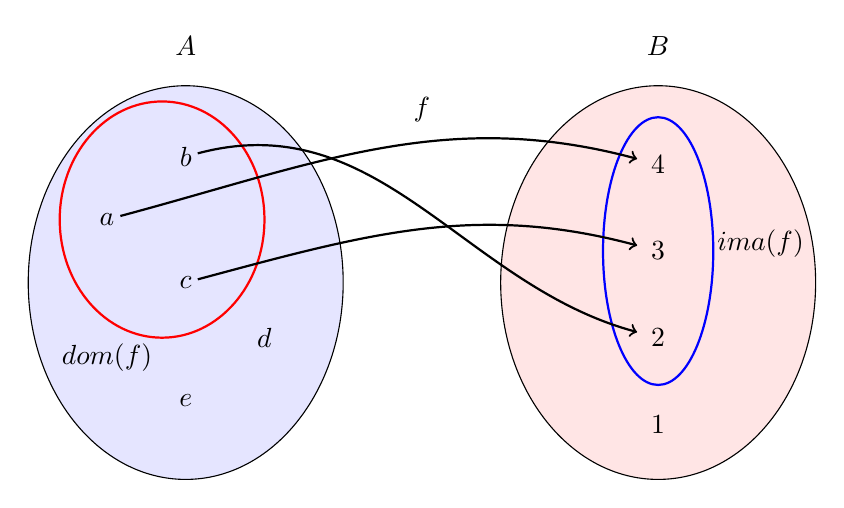
\begin{tikzpicture}
		\draw[fill=blue!10] (0,0) ellipse (2cm and 2.5cm); 		  % Primeiro conjunto
		\node at (0,3) {$A$};									                  % Rótulo do primeiro conjunto
		\draw[fill=red!10] (6,0) ellipse (2cm and 2.5cm);  		  % Segundo conjunto
		\node at (6,3) {$B$};									                  % Rótulo do segundo conjunto
		\draw[red, thick] (-0.3,0.8) ellipse (1.3cm and 1.5cm);	% Domínino da função f
		\node at (-1,-0.95) {$dom(f)$};							            % Rótulo do domínio de f
		\draw[blue, thick] (6,0.4) ellipse (0.7cm and 1.7cm);	  % Imagem da função f
		\node at (7.3,0.5) {$ima(f)$};							            % Rótulo do imagem de f
		\node at (3,2.2) {$f$};		
		% Elementos do primeiro conjunto
		\node[inner sep=2pt] (a1) at (-1,0.8) {$a$};
		\node[inner sep=2pt] (a2) at (0,1.6) {$b$};
		\node[inner sep=2pt] (a3) at (0,0) {$c$};
		\node[inner sep=2pt] (a4) at (1,-0.7) {$d$};
		\node[inner sep=2pt] (a5) at (0,-1.5) {$e$};
		% Elementos do segundo conjunto
		\node[inner sep=2pt] (b1) at (6,1.5) {$4$};
		\node[inner sep=2pt] (b2) at (6,0.4) {$3$};
		\node[inner sep=2pt] (b3) at (6,-0.7) {$2$};
		\node[inner sep=2pt] (b4) at (6,-1.8) {$1$};
		% Setas
		\draw[->, shorten >=3pt, thick] (a1) to[out=15,in=165] (b1);
		\draw[->, shorten >=3pt, thick] (a2) to[out=15,in=165] (b3);
		\draw[->, shorten >=3pt, thick] (a3) to[out=15,in=165] (b2);
	\end{tikzpicture}
	\caption{Diagrama de uma função $f$ qie é injetora.}
	\label{fig:FuncaoInjetora1}	
\end{figure}

\begin{figure}[H]
	\centering
	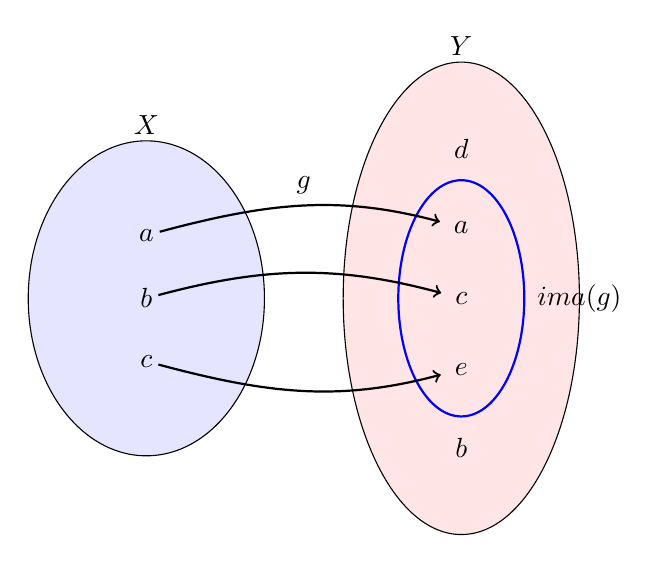
\begin{tikzpicture}
		\draw[fill=blue!10] (0,0) ellipse (1.5cm and 2cm);			% Conjunto X
		\node at (0,2.2) {$X$};										% Rótulo X
		\draw[fill=red!10] (4,0) ellipse (1.5cm and 3cm);			% Conjunto Y
		\draw[blue, thick] (4,0) ellipse (0.8cm and 1.5cm);			% Imagem da função g
		\node at (4,3.2) {$Y$};										% Rótulo Y
		\node[above] at (2,1.2) {$g$};								% Rótulo g
		\node at (5.5,0) {$ima(g)$};								% Rótulo do image de g
		
		% Elementos de X
		\node[inner sep=2pt] (x1) at (0,0.8) {$a$};
		%\node[draw,circle,fill=white,inner sep=2pt] (x2) at (0,0) {$b$};
		\node[inner sep=2pt] (x2) at (0,0) {$b$};
		\node[inner sep=2pt] (x3) at (0,-0.8) {$c$};
		% Elementos de Y
		\node[inner sep=2pt] (y1) at (4.0,0.9) {$a$};
		\node[inner sep=2pt] (y2) at (4.0,0) {$c$};
		\node[inner sep=2pt] (y3) at (4.0,1.9) {$d$};
		\node[inner sep=2pt] (y4) at (4.0,-0.9) {$e$};
		\node[inner sep=2pt] (y5) at (4.0,-1.9) {$b$};
		% Setas
		\draw[->, shorten >=3pt, thick] (x1) to[out=15,in=165]  (y1);
		\draw[->, shorten >=3pt, thick] (x2) to[out=15,in=165]  (y2);
		\draw[->, shorten >=3pt, thick] (x3) to[out=-15,in=195] (y4);
	\end{tikzpicture}
	\caption{Diagrama de uma função injetora $g$.}
	\label{fig:FuncaoInjetora2}	
\end{figure}

\begin{figure}[H]
	\centering
	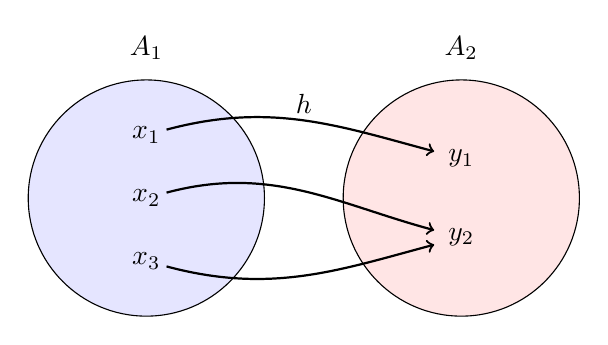
\begin{tikzpicture}
		\draw[fill=blue!10] (0,0) ellipse (1.5cm and 1.5cm);			% Conjunto A
		\node at (0,1.9) {$A_1$};										% Rótulo A1
		\draw[fill=red!10] (4,0) ellipse (1.5cm and 1.5cm);				% Conjunto B
		\node at (4,1.9) {$A_2$};										% Rótulo A2
		\node[above] at (2,0.95) {$h$};									% Rótulo h
		
		% Elementos
		\node[inner sep=2pt] (x1) at (0,0.8) {$x_1$};
		\node[inner sep=2pt] (x2) at (0,0) {$x_2$};
		\node[inner sep=2pt] (x3) at (0,-0.8) {$x_3$};
		
		\node[inner sep=2pt] (y1) at (4.0,0.5) {$y_1$};
		\node[inner sep=2pt] (y2) at (4.0,-0.5) {$y_2$};
		
		% Setas
		\draw[->, shorten >=3pt, thick] (x1) to[out=15,in=165]  (y1);
		\draw[->, shorten >=3pt, thick] (x2) to[out=15,in=165]  (y2);
		\draw[->, shorten >=3pt, thick] (x3) to[out=-15,in=195] (y2);
	\end{tikzpicture}
	\caption{Diagrama de uma função $h$, que não é injetora.}
	\label{fig:FuncaoInjetora3}	
\end{figure}

\begin{exemplo}\label{exe:FuncoesInjetora1}
	As funções:
	\begin{itemize}
		\item[$(a)$] $f(x) = 2x$ com $f \in \mathbb{R}^\mathbb{Z}$.
		\item[$(b)$] $g(x) = 3x + 1$ com $g \in \mathbb{Z}^\mathbb{Z}$.
    \item[$(c)$] A função de Cantor $C(x, y) = \frac{(x + y)(x + y + 1)}{2} + b$ com $C \in \mathbb{N}^{\mathbb{N} \times \mathbb{N}}$.
    \item[$(d)$] $Step_k(x) = x + k$ com $k \in \mathbb{Z}_+^*$ e $Step_k \in \mathbb{Z}^\mathbb{Z}$.
	\end{itemize} 
	são todas injetoras. Por outro lado, as funções a seguir não são injetoras.
	\begin{itemize}
		\item[$(e)$] $T(x, y) = xy$ com $T \in \mathbb{B}^{\mathbb{B} \times \mathbb{B}}$ e $\mathbb{B} = \{0,1\}$.
		\item[$(f)$] $C(x, y) = min(x, y)$ com $C \in L^{L \times L}$ e $L = \{x \in \mathbb{R} \mid 0 \leq x \leq 1\}$.
		\item[$(g)$] $h(x) = x^2$ com $h \in \mathbb{Z}^\mathbb{Z}$.
	\end{itemize} 
\end{exemplo}

Pela Definição \ref{def:FuncaoInjetora} pode-se notar que a propriedade de injeção de uma função $f$ é uma propriedade relacionada diretamente com os ``dados'' de entrada que a função recebe, isto é, a propriedade de injeção está diretamente ligado ao conjunto $dom(f)$. A próxima propriedade que será apresentada, por sua vez, está relacionada ao dados que a função produz após sua aplicação, a mesma relaciona o dados de saída com o conjunto de chega da assinatura da função.


\begin{figure}[h]
	\centering
	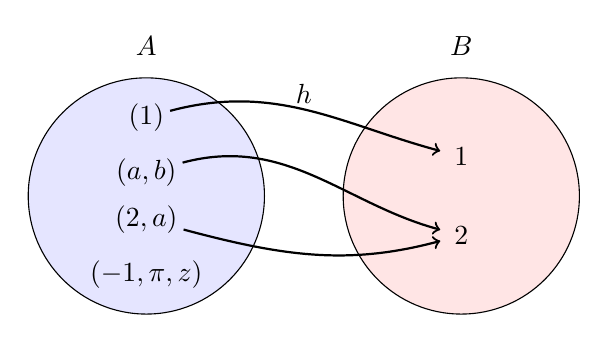
\begin{tikzpicture}
		\draw[fill=blue!10] (0,0) ellipse (1.5cm and 1.5cm);			% Conjunto A
		\node at (0,1.9) {$A$};											% Rótulo A
		\draw[fill=red!10] (4,0) ellipse (1.5cm and 1.5cm);				% Conjunto B
		\node at (4,1.9) {$B$};											% Rótulo B
		\node[above] at (2,1.05) {$h$};									% Rótulo h
		
		% Elementos
		\node[inner sep=2pt] (x1) at (0,1) 			{$(1)$};
		\node[inner sep=2pt] (x2) at (0,0.3) 	 	{$(a, b)$};
		\node[inner sep=2pt] (x3) at (0,-0.3)		{$(2, a)$};
		\node[inner sep=2pt] (x4) at (0,-1.0)		{$(-1, \pi, z)$};
		
		\node[inner sep=2pt] (y1) at (4.0,0.5) 	{$1$};
		\node[inner sep=2pt] (y2) at (4.0,-0.5) {$2$};
		
		% Setas
		\draw[->, shorten >=3pt, thick] (x1) to[out=15,in=165]  (y1);
		\draw[->, shorten >=3pt, thick] (x2) to[out=15,in=165]  (y2);
		\draw[->, shorten >=3pt, thick] (x3) to[out=-15,in=195] (y2);
	\end{tikzpicture}
	\caption{Diagrama de uma função $h$ que é sobrejetora.}
	\label{fig:FuncaoSobrejetora1}	
\end{figure}

\begin{definicao}[Função sobrejetora]\label{def:FuncaoSobrejetora}
	Seja $f \in B^A$, $f$ é dita ser \textbf{sobrejetora} sempre que para todo $y \in B$ existe $x \in A$ tal que $f(x) = y$.
\end{definicao}

Outra caracterização para funções sobrejetora apresentada em \cite{lipschutz1971-Topo} é que, uma função $f \in B^A$ é sobrejetora sempre que $\overrightarrow{f}[dom(f)] = B$, porém, dizer isso é o mesmo que dizer que,  uma função $f \in B^A$ é sobrejetora sempre que $ima(f) = B$, que é outra forma de caracterizar funções sobrejetoras como dito em \cite{carmo2013}. Claramente a função descrita na Figura \ref{fig:FuncaoInjetora3} e \ref{fig:FuncaoSobrejetora1} são ambas sobrejetoras, enquanto as funções esboçadas nas Figuras \ref{fig:FuncaoInjetora1} e \ref{fig:FuncaoInjetora2} não são sobrejetoras, são também exemplos de funções sobrejetoras os itens $(d), (e)$ e $(f)$ do Exemplo \ref{exe:FuncoesInjetora1}.

\begin{exemplo}\label{exe:FuncaoSobrejetora}
	As funções,
	\begin{itemize}
		\item[$(a)$] $f(x) = 2x$ com $f \in \mathbb{P}^\mathbb{N}$.
		\item[$(b)$] $g(x) = \displaystyle\frac{1}{x}$ com $g \in L_0^{\mathbb{N}}$ onde $L_0 = \{x \in \mathbb{R} \mid 0 < x \leq 1\}$.
	\end{itemize} 
	são funções sobrejetoras. Por outro lado, as funções,
	\begin{itemize}
		\item[$(c)$] $A(x) = 1 - x$ com $A \in \mathbb{N}^\mathbb{N}$.
		\item[$(d)$] $B(x) = 2x$ com $B \in \mathbb{Z}^\mathbb{N}$.
	\end{itemize}
	não são funções sobrejetoras.
\end{exemplo}

\begin{definicao}[Função bijetora]\label{def:FuncaoBijetora}
	Seja $f \in B^A$, $f$ é dita ser \textbf{bijetora} sempre que $f$ for total, injetora e sobrejetora.
\end{definicao}

As funções bijetoras como dito em \cite{lipschutz1971-Topo}, também costuma ser chamadas de funções biunívocas ou mapeamento um para um (ou \textit{one-to-one} em inglês \cite{carmo2013}). Nos casos em que a bijeção $f \in A^A$ para algum conjunto $A$, a função bijetora $f$ costuma ser chamada de permutação \cite{carmo2013} sobre (ou em) A. 

\begin{exemplo}\label{exe:FuncaoIdentidade}
  Seja $A$ um conjunto, a função identidade $id_A : A \rightarrow A$ construída por $id_A(x) = x$ para todo $x \in A$ é claramente uma bijeção.
\end{exemplo}

\begin{exemplo}
  A função descrita pela Figura \ref{fig:FuncaoBijetora1} é claramente uma bijeção, uma vez que é visivelmente uma função de um para um.
\end{exemplo}

\begin{figure}[H]
	\centering
	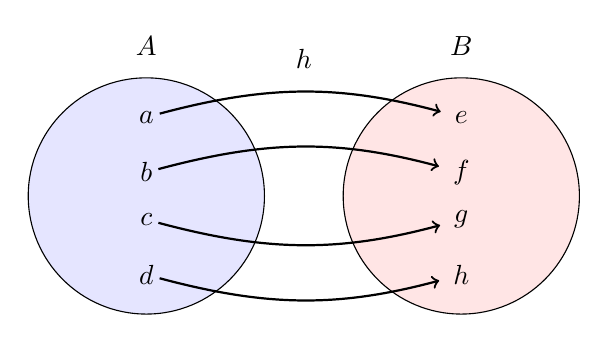
\begin{tikzpicture}
		\draw[fill=blue!10] (0,0) ellipse (1.5cm and 1.5cm);			% Conjunto A
		\node at (0,1.9) {$A$};											% Rótulo A
		\draw[fill=red!10] (4,0) ellipse (1.5cm and 1.5cm);				% Conjunto B
		\node at (4,1.9) {$B$};											% Rótulo B
		\node[above] at (2,1.5) {$h$};									% Rótulo h
		
		% Elementos
		\node[inner sep=2pt] (x1) at (0,1) 			{$a$};
		\node[inner sep=2pt] (x2) at (0,0.3) 	 	{$b$};
		\node[inner sep=2pt] (x3) at (0,-0.3)		{$c$};
		\node[inner sep=2pt] (x4) at (0,-1.0)		{$d$};
		
		\node[inner sep=2pt] (y1) at (4,1) 			{$e$};
		\node[inner sep=2pt] (y2) at (4,0.3) 	 	{$f$};
		\node[inner sep=2pt] (y3) at (4,-0.3)		{$g$};
		\node[inner sep=2pt] (y4) at (4,-1.0)		{$h$};

		% Setas
		\draw[->, shorten >=3pt, thick] (x1) to[out=15,in=165]  (y1);
		\draw[->, shorten >=3pt, thick] (x2) to[out=15,in=165]  (y2);
		\draw[->, shorten >=3pt, thick] (x3) to[out=-15,in=195] (y3);
    \draw[->, shorten >=3pt, thick] (x4) to[out=-15,in=195] (y4);
	\end{tikzpicture}
	\caption{Diagrama de uma função $h$ que é bijetora.}
	\label{fig:FuncaoBijetora1}	
\end{figure}

\begin{exemplo}
  São bijetoras.
  \begin{itemize}
    \item[(a)] A função $f(x) = 2x + 1$ com $f: \mathbb{R} \rightarrow \mathbb{R}$.
    \item[(b)] A função\footnote{$exp(x)$ é a forma padrão usada principalmente em linguagens de programação e calculadoras científicas para denotar a função exponencial, que na matemática é escrita como $e^x$ sendo $e$ a constante do logaritmo natural.} $exp(x)$ com $exp: \mathbb{R} \rightarrow \mathbb{R}_+$.
    \item[(c)] A função $C$ de Cantor, esboçada no item $(c)$ do Exemplo \ref{exe:FuncoesInjetora1} é uma bijeção.
    \item[(d)] A função $r(x) = -x$  com $r \in \mathbb{Z}^\mathbb{Z}$ é também uma bijeção\footnote{A função $r$ em algumas obra costuma ser chamada de função de inversão de sinal, pois ela manda todo inteiro positivo $x$ em seu correspondente $-x$, e manda todo $-x$ em sua contraparte positiva.}.
  \end{itemize}
\end{exemplo}

\section{Composição e Função Inversa}\label{sec:FuncaoInversa}

Como qualquer outro objeto matemático, também existem operações sobre as funções, isto é, mecanismos que atuam sobre funções para criar novas funções. Dessa operações a mais importante é sem dúvidas a composição de funções.

\begin{definicao}[Composição de função]\label{def:ComposicaoFuncional}
	Sejam $f: A \rightarrow B$ e $g: B \rightarrow C$ duas funções, a função composta de $g$ com $f$, denotada por $g \circ f$, é uma função com a assinatura $g \circ f: A \rightarrow C$ que atende as seguintes restrições:
	\begin{itemize}
		\item $dom(g \circ f) = \{x \mid x \in dom(f) \land f(x) \in dom(g)\}$ e 
		\item $(\forall x \in dom(g \circ f))[(g \circ f)(x) = g(f(x))]$.
	\end{itemize}
\end{definicao}

Se as funções $f: A \rightarrow B$ e $g: B \rightarrow C$ forem enxergadas apenas como mapeamentos, a composição  das duas funções pode ser vista como sendo uma forma de mapear elementos de $A$ direto em elementos de $C$, sem há necessidade (explícita) de mapear em $B$, como ilustrado na Figura \ref{fig:FuncaoComposta}.

\begin{figure}[H]
	\centering
	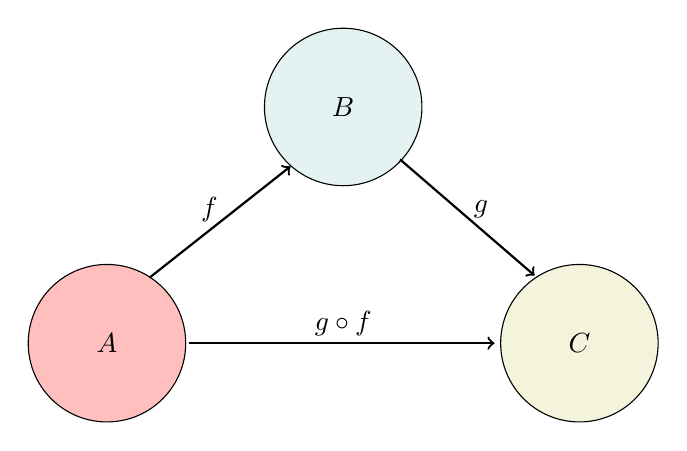
\begin{tikzpicture}
		% Conjunto A
		\draw[fill=pink] (0,0) ellipse (1.0cm and 1.0cm);
		\node at (0,0) {$A$};
		% Conjunto B
		\draw[fill=olive!10] (6,0) ellipse (1.0cm and 1.0cm);
		\node at (6,0) {$C$};
		% Conjunto C
		\draw[fill=teal!10] (3,3) ellipse (1.0cm and 1.0cm);
		\node at (3,3) {$B$};

		% Rótulo das funções
		\node at (1.3,1.7) 	{$f$};
		\node at (4.75,1.7) {$g$};
		\node at (3,0.25) 	{$g \circ f$};

		% Pontos para as setas
		\node[inner sep=1pt] (xA) at (0.5,0.8)				{ };
		\node[inner sep=1pt] (aA) at (1.0,0)					{ };
		\node[inner sep=1pt] (yB) at (2.4,2.3)				{ };
		\node[inner sep=1pt] (xB) at (3.68,2.37)			{ };
		\node[inner sep=1pt] (yC) at (5.5,0.8)				{ };
		\node[inner sep=1pt] (bC) at (5,0)						{ };

		% Setas
		\draw[->, shorten >=1pt, thick] (xA) to  (yB);
		\draw[->, shorten >=1pt, thick] (xB) to  (yC);
		\draw[->, shorten >=1pt, thick] (aA) to  (bC);
	\end{tikzpicture}
	\caption{Diagrama da composição de uma função $g$ com outra função $f$.}
	\label{fig:FuncaoComposta}	
\end{figure}

Por outro lado, a composição vista enquanto máquina (ou caixa preto), e na verdade uma máquina ``maior'', em que, as funções usadas na composição são apenas partes aninhadas sequencialmente, a Figura \ref{fig:FuncaoCompostaBlackBox} apresenta essa ideia.

\begin{figure}[h]
	\centering
	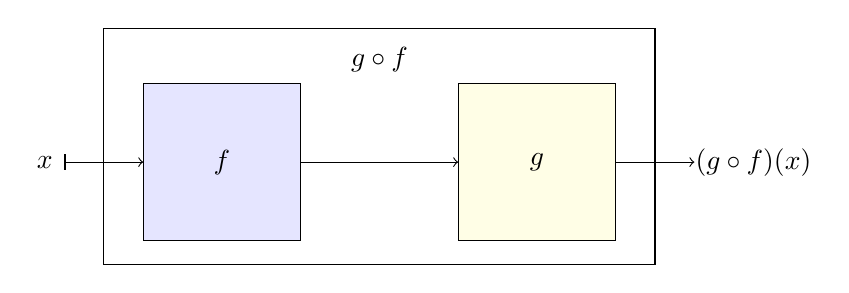
\begin{tikzpicture}
    % Desenhando e pintando os blocos internos
    \fill[blue!10] (0,0) rectangle (2,2);
    \draw (0,0) rectangle (2,2);
    \fill[yellow!10] (4,0) rectangle (6,2);
    \draw (4,0) rectangle (6,2);
    % Desenhando o bloco externo
    \draw (-0.5,-0.3) rectangle (6.5,2.7);
    % Inserido as setas
		\draw[->]  (2,1) -- (4,1);
    \draw[|->] (-1, 1) -- (0,1);
    \draw[->]  (6,1) -- (7,1);
    % Escrevendo os símbolos
    \node (a) at (1,1)      {$f$};
    \node (b) at (5,1)      {$g$};
    \node (c) at (3,2.3)    {$g \circ f$};
    \node (d) at (-1.25, 1)  {$x$};
    \node (e) at (7.75, 1)   {$(g \circ f)(x)$};
	\end{tikzpicture}
	\caption{Composição $g \circ f$ vista enquanto uma máquina (ou caixa preta).}
	\label{fig:FuncaoCompostaBlackBox}
\end{figure}


Agora dado duas funções $f: A \rightarrow B$ e $g: B \rightarrow C$, com $A$ e $B$ sendo conjuntos numéricos e $f(x) = E$ e $g(x') = E'$ onde $E$ e $E'$ são expressões válidas, e além disso, a expressão $E$ sendo capaz de descrever os elementos em $dom(g)$, tem-se que $(g \circ f)(x) = E'[E/x']$, onde $E'[E/x']$ será uma nova expressão válida obtida a partir da substituição na expressão $E'$ de todas as ocorrências da variável $x'$ pela expressão $E$.

\begin{exemplo}\label{exe:ComposicaoFuncao1}
	Dado a função de naturais em reais $f(x) = \frac{1}{x+1}$, e a função de reais em reais $g(x) = (-x + 2)^3 + 4$, tem-se que,
	\begin{eqnarray*}
		dom(f) & = & \mathbb{N}\\
		dom(g) & = & \mathbb{R}
	\end{eqnarray*}
	além disso, tem-se a composição: 
	$$(g \circ f)(x) = \Big(- \frac{1}{x+1} + 2\Big)^3 + 4$$
	note agora que
	\begin{eqnarray*}
		dom(g \circ f) & = & \{x \mid x \in dom(f) \land f(x) \in dom(g)\}\\ 
		& = & \{x \mid x \in \mathbb{N} \land f(x) \in \mathbb{R}\}\\
		& = & \mathbb{N}
	\end{eqnarray*}
	e, portanto, a composição $g \circ f$ é uma construção válida.
\end{exemplo}

\begin{exemplo}\label{exe:ComposicaoFuncao2}
	Dado duas funções $f_1, f_2 \in \mathbb{Z}^{\mathbb{Z}}$ sendo que $f_1(x) = -x + 3$ e $f_2(x) = 2x + 1$, tem-se que $dom(f_1)  =  \mathbb{Z}$ e $dom(f_2)  =  \mathbb{Z}$ assim tem-se que,
	\begin{itemize}
		\item[(a)] $(f_1 \circ f_2)(x) = -2x + 2$ e
		\item[(b)] $(f_2 \circ f_1)(x) = -2x + 7$.
	\end{itemize}
	note agora que,
	\begin{eqnarray*}
		dom(f_1 \circ f_2) & = & \{x \mid x \in dom(f_2) \land f_2(x) \in dom(f_1)\}\\ 
		& = & \{x \mid x \in \mathbb{Z} \land f_1(x) \in \mathbb{Z}\}\\
		& = & \mathbb{Z}
	\end{eqnarray*}
	além disso, 
	\begin{eqnarray*}
		dom(f_2 \circ f_1) & = & \{x \mid x \in dom(f_1) \land f_1(x) \in dom(f_2)\}\\ 
		& = & \{x \mid x \in \mathbb{Z} \land f_1(x) \in \mathbb{Z}\}\\
		& = & \mathbb{Z}
	\end{eqnarray*}
	e, portanto, as composições $f_1 \circ f_2$ e $f_2 \circ f_1$ são ambas construções válidas.
\end{exemplo}

O Exemplo \ref{exe:ComposicaoFuncao2} é interessante pois ele mostra que a composição de funções não é uma operação comutativa, no sentido de igualdade, ou seja, não é sempre que ocorre que $f_1 \circ f_2 = f_2 \circ f_1$. 

\begin{exemplo}\label{exe:ComposicaoFuncao3}
	Dado duas funções $i: \mathbb{N} \rightarrow \mathbb{Z}$ e $Id_\mathbb{Z} : \mathbb{Z} \rightarrow \mathbb{Z}$ tal que $i(x) = -x$ e $j(x) = \sqrt{x}$, tem-se que a composição $Id_\mathbb{Z} \circ i$ não é uma composição válido, pois por definição a aplicação para algum $x \in \mathbb{N}$ seria da forma $(Id_\mathbb{Z} \circ i)(x) = Id_\mathbb{Z}(i(x)) = \sqrt{-x}$, e obviamente, $\sqrt{-x}$ não é uma expressão válida no contexto dos números inteiros. Note que neste exemplo isso ocorre pelo fato de $-x \notin dom(g)$ com $x \in \mathbb{N}$.
\end{exemplo}

\begin{exemplo}\label{exe:ComposicaoFuncao4}
  Dado a função $f(x) = x + 1$ e $g(x) = x - 1$ com $f: \mathbb{N} \rightarrow \mathbb{N}$ e $g: \mathbb{Z} \rightarrow \mathbb{Z}$, tem-se que $(g \circ f)(x) = g(f(x)) = x$, por outro lado, $f \circ g$ não é um composição válida, pois basta notar que $0 \in dom(g)$, mas $g(0) \notin dom(f)$\footnote{Este exemplo considera que $\mathbb{N} \subseteq \mathbb{Z}$ através da ideia de sobrecarga de símbolo, ou seja, todo número natural é sobrecarregado para ser considerado também como número inteiro positivo.}. 
\end{exemplo}

\begin{proposicao}\label{prop:AssociativaComposicaoFuncao}
  A composição de funções é associativa.
\end{proposicao}

\begin{proof}
  Considere que $f \in B^A, g \in C^B$ e $h \in D^C$, agora pela Definição \ref{def:ComposicaoFuncional} se a composição entre essas funções existe ela irá satisfazer as seguintes pertinência, $g \circ f \in C^A$ e $h \circ (g \circ f) \in D^A$, por outro lado, $h \circ g \in D^B$ e $(h \circ g) \circ f \in D^A$, ou seja, ambas as composições estão no mesmo espaço funcional. Além disso, tem-se que:
	\begin{eqnarray*}
		dom(h \circ (g \circ f)) & \stackrel{Def. \ref{def:ComposicaoFuncional}}{=} & \{x \mid x \in dom(g \circ f) \land (g \circ f)(x) \in dom(h)\}\\
		& \stackrel{Def. \ref{def:ComposicaoFuncional}}{=} & \{x \mid x \in \{y \mid y \in dom(f) \land f(y) \in dom(g)\}\\ 
		& & \land \ (g \circ f)(x) \in dom(h)\}\\
		& = & \{x \mid x \in dom(f) \land f(x) \in dom(g) \land g(f(x)) \in dom(h)\}
	\end{eqnarray*}
	Por outro lado, tem-se que:
	\begin{eqnarray*}
		dom((h \circ g) \circ f) & \stackrel{Def. \ref{def:ComposicaoFuncional}}{=} & \{x \mid x \in dom(f) \land f(x) \in dom(h \circ g)\}\\
		& \stackrel{Def. \ref{def:ComposicaoFuncional}}{=} & \{x \mid x \in dom(f) \land\\ 
		& & f(x) \in \{y \mid y \in dom(g) \land g(y) \in dom(h)\} \}\\
		& = & \{x \mid x \in dom(f) \land f(x) \in dom(g) \land g(f(x)) \in dom(h)\}
	\end{eqnarray*}
	consequentemente, $dom(h \circ (g \circ f)) = dom((h \circ g) \circ f)$, por fim note que para todo $x \in dom(f)$ segue que,
	\begin{eqnarray*}
		(h \circ (g \circ f))(x) & = & h( (g \circ f)(x))\\
		& = & h(g(f(x)))\\
		& = & (h \circ g)(f(x))\\
		& = & ((h \circ g) \circ f)(x)
	\end{eqnarray*}
	o que conclui a prova.
\end{proof}

A seguir são apresentados mais alguns resultados sobre a composição de funções.

\begin{teorema}\label{teo:InversaEsquerda}
	Se $f \in B^A$ é uma função injetora, então existe uma função $g \in A^B$ tal que $(g \circ f)(x) = x$.
\end{teorema}

\begin{proof}
	Suponha que $f \in B^A$ é uma função injetora, agora deixe $y \in B$. Agora defina uma nova função $g \in B^A$ da seguinte forma:
	\begin{eqnarray*}
		g(y) = \left\{\begin{array}{ll}
			x, & \text{se } f(x) = y\\
			a, & \text{senão}
		\end{array}\right.
	\end{eqnarray*}
	para algum $x \in dom(f)$ e $a \in A$. Note que se $y \in ima(f)$, então por $f$ ser injetora irá existir $x \in A$ tal que $f(x) = y$, no caso contrário, é claro que o resultado para $g(y)$ será um $a \in A$ predefinido (ou pré-escolhido), de forma que $g$ é claramente uma função total. Agora note que para todo $x \in dom(f)$ é claro pela contrução de $g$ que $(g \circ f)(x) = g(f(x)) = x$.
\end{proof}

\begin{teorema}\label{teo:InversaDireta}
	Se $f \in B^A$ é uma função sobrejetora, então existe uma função $g \in A^B$ tal que $(f \circ g)(y) = y$.
\end{teorema}

\begin{proof}
	A demonstração fica como exercício ao leitor.
\end{proof}

\begin{teorema}\label{teo:ComposicaoFuncaoPreservaTipo}
	Sejam $f \in B^A$ e $g \in C^B$ duas funções totais, tem-se que:
	\begin{itemize}
		\item[$i$.] Se $f$ e $g$ são injetoras, então $g \circ f$ também é injetora.
		\item[$ii$.] Se $f$ e $g$ são sobrejetoras, então $g \circ f$ também é sobrejetoras.
	\end{itemize}
\end{teorema}

\begin{proof}
	Dado duas funções totais $f \in B^A$ e $g \in C^B$ tem-se:
	\begin{itemize}
		\item[$i$.] Suponha que $f$ e $g$ são injetoras, desde que $f$ é total tem-se que para todo $a, a' \in A$ que $f(a)$ e $f(a')$ estão definidos, além disso, como por hipótese $f$ é injetora tem-se para $a \neq a'$ que $f(a) \neq f(a')$, agora por definição de $g \circ f$ todo $f(x) \in ima(f)$ é tal que $f(x) \in dom(g)$, logo $f(a), f(a') \in dom(g)$, como por hipótese $g$ é injetora tem-se que $g(f(a)) \neq g(f(a'))$, ou seja, tem-se que $(g \circ f)(a) \neq (g \circ f)(a')$ e, portanto, $g \circ f$ também é injetora.
		\item[$ii$.] A demostração desde item ficará com exercício ao leitor.
	\end{itemize}
\end{proof}

\begin{corolario}\label{col:ComposicaoFuncaoPreservaTipo}
	Se $f \in B^A$ e $g \in C^B$ são bijetoras, então $g \circ f$ também é bijetora.
\end{corolario}

\begin{proof}
	Direto do Teorema \ref{teo:ComposicaoFuncaoPreservaTipo}.
\end{proof}

\begin{teorema}\label{teo:NeutralidadeDaFuncaoIdentidade}
	Dado uma função $f \in B^A$, tem-se que $f \circ id_A = f$ e $id_B \circ f = f$.
\end{teorema}

\begin{proof}
	Dado uma função qualquer $f \in B^A$ tem-se para todo $x \in dom(f)$ que, 
	\begin{eqnarray*}
		(f \circ id_A)(x) = f(id_A(x)) = f(x)
	\end{eqnarray*}
	ou seja, $f \circ id_A = f$. Por outro lado, considere que para $x \in dom(f)$ tem-se que $f(x) = y$ assim,
	\begin{eqnarray*}
		(id_B \circ f)(x) = id_B(f(x)) = id_B(y) = y = f(x)
	\end{eqnarray*}
	consequentemente, $id_B \circ f = f$.
\end{proof}

A partir dos conceitos de composição de funções e de funções bijetoras, é possível definir o conceito de inversão para a teoria das funções, ou seja, apresentar o conceito de função inversa. De um ponto de vista operacional, uma função inversa ``desfaz'' as ações realizadas por uma outra função. A existência da função inversa de funções bijetoras é um corolário direto dos Teoremas \ref{teo:InversaEsquerda} e \ref{teo:InversaDireta} com dito esboçado em \cite{zach2021-TC}.

\begin{definicao}[Função Inversa]\label{def:FuncaoInversa}
	Seja $f \in B^A$ uma bijeção, uma função inversa de $f$ é qualquer função $g \in A^B$ tal que $g \circ f = id_{dom(f)}$ e $f \circ g = id_{ima(f)}$, ou seja, para todo $x \in dom(f), y \in ima(f)$ tem-se que $(g \circ f)(x) = x$ e $(f \circ g)(y) = y$.
\end{definicao}

Agora dado que toda bijeção $f$ é uma função total, as igualdades expressas na Definição \ref{def:FuncaoInversa} podem ser reescritas como sendo da forma $g \circ f = id_{A}$ e $f \circ g = id_{B}$.

\begin{nota}[Apelido da inversa]
  Dado uma função $f \in B^A$, na literatura (ver \cite{lipschutz1978-TC, lipschutz2013-MD}) é comum usar $f^{-1}$ para se referir a função inversa de $f$. Além disso, como discutido em \cite{carmo2013} se $f \in B^A$ é uma bijeção sua inversa também será uma bijeção.
\end{nota}

\begin{exemplo}\label{exe:FuncaoInversa1}
	Para $f \in \mathbb{R}^\mathbb{R}$ com $f(x) = 3x + 4$ tem-se $f^{-1}(x) = \frac{(x - 4)}{3}$.
\end{exemplo}

\begin{exemplo}\label{exe:FuncaoInversa2}
	Para $f \in ]0,1]^{\mathbb{R}^*_+}$ com $f(x) = \frac{1}{x}$ tem-se $f^{-1}(x) = \frac{1}{x}$.
\end{exemplo}

\begin{exemplo}\label{exe:FuncaoInversa3}
	Seja $\mathbb{L}$ o conjunto de todas as listas de números inteiros, a função $doubleend \in \mathbb{L}^\mathbb{L}$ que dubplica o último elemento na lista $l$, tem como inversa a função $delatend \in \mathbb{L}$ que apaga o último elemento de uma lista.
\end{exemplo}

\begin{exemplo}\label{exe:FuncaoInversa4}
	Para $f \in \mathbb{N}^\mathbb{Z}$ com, 
	\begin{eqnarray*}
		f(x) = \left\{\begin{array}{ll}
			2x, & \text{se } x \geq 0\\
			-2x - 1, & \text{senão}
		\end{array}\right.
	\end{eqnarray*}
	tem-se então que $f^{-1} \in \mathbb{Z}^\mathbb{N}$ sendo da forma,
	\begin{eqnarray*}
		f^{-1}(x) = \left\{\begin{array}{ll}
			\frac{x}{2}, & \text{se } x \in \mathbb{P}\\
			-\frac{(x + 1)}{2}, & \text{senão}
		\end{array}\right.
	\end{eqnarray*}
\end{exemplo}

\begin{teorema}
	Se $f \in B^A$ e $g \in C^B$ são bijetoras, então $(g \circ f)^{-1} = f^{-1} \circ g^{-1}$.
\end{teorema}

\begin{proof}
	Suponha que $f \in B^A$ e $g \in C^B$ são bijetoras, logo pelo Corolário \ref{col:ComposicaoFuncaoPreservaTipo} tem-se que $g \circ f$ também é uma bijeção e dado que $g \circ f \in C^A$ tem-se que $(g \circ f)^{-1} \in A^C$, assim,
	\begin{eqnarray*}
		(g \circ f)^{-1} & \stackrel{Teo. \ref{teo:NeutralidadeDaFuncaoIdentidade}}{=} &  (g \circ f)^{-1} \circ id_C\\
		& \stackrel{Def. \ref{def:FuncaoInversa}}{=} & (g \circ f)^{-1} \circ (g \circ g^{-1})\\
		& \stackrel{Prop. \ref{prop:AssociativaComposicaoFuncao}}{=} & ((g \circ f)^{-1} \circ g) \circ g^{-1}\\
		& \stackrel{Teo. \ref{teo:NeutralidadeDaFuncaoIdentidade}}{=} & ((g \circ f)^{-1} \circ (g \circ id_B)) \circ g^{-1}\\
		& \stackrel{Def. \ref{def:FuncaoInversa}}{=} & ((g \circ f)^{-1} \circ (g \circ (f \circ f^{-1}))) \circ g^{-1}\\
		& \stackrel{Prop. \ref{prop:AssociativaComposicaoFuncao}}{=} & ((g \circ f)^{-1} \circ ((g \circ f) \circ f^{-1})) \circ g^{-1}\\
		& \stackrel{Prop. \ref{prop:AssociativaComposicaoFuncao}}{=} & (((g \circ f)^{-1} \circ (g \circ f)) \circ f^{-1}) \circ g^{-1}\\
		& \stackrel{Def. \ref{def:FuncaoInversa}}{=} & (id_A \circ f^{-1}) \circ g^{-1}\\
		& \stackrel{Prop. \ref{prop:AssociativaComposicaoFuncao}}{=} & id_A \circ (f^{-1} \circ g^{-1})
	\end{eqnarray*}
	agora desde que $f^{-1} \in A^B$ e $g^{-1} \in B^C$, tem-se que $f^{-1} \circ g^{-1} \in A^C$ e assim pelo Teorema \ref{teo:NeutralidadeDaFuncaoIdentidade} tem-se que $id_A \circ (f^{-1} \circ g^{-1}) = f^{-1} \circ g^{-1}$, o que completa a prova.
\end{proof}

\section{Famílias}

Halmos em \cite{halmos2001} menciona que, ``. . . existem diversas ocasiões em que a imagem de uma função é tida como mais importante do que a própria função''. Quando este é o caso, a terminologia e a notação, ambas, passam por radicais alterações, que serão introduzidas a seguir.

\begin{definicao}[Família Indexada]\label{def:Familia}
	Sejam $I$ e $D$ dois conjuntos não vazios, uma família indexada (ou simplesmente família) por $I$ de elementos de $D$, é uma função injetora e total $u: I \rightarrow D$.
\end{definicao}

A Definição \ref{def:Familia} estabelece o conceito de família\footnote{Obras como \cite{halmos2001} e \cite{carmo2013} também mencionam a nomeclatura indexaçõe.}, a ideia aqui decorre da seguinte forma, existe um conjunto de índices (ou endereços) $I$ e um conjunto de dados $D$, a família $u$ é então uma forma de organizar via uso de índices\footnote{Ou seja, uma família estabelece o conceito de chave-valor, tão importante dentro das linguagens de programação.} $i \in I$ os elementos armazendos $d \in D$. Aqui cada $u(i)$ é escrito na verdade como $u_i$, e é chamado de $i$-ésimo elemento da família. Além disso, a família é representado como $(u_i)_{i \in I}$, em vez de simplesmente usar o símbolo $u$. 

Uma classe de famílias bastante importante na matemática, e por extensão na ciência da computação, são as família ditas como sendo \textbf{sequenciais}, esta famílias apresentam a característica de que seu conjunto de índices $I$ é obrigatóriamente uma estrutura de conjunto totalmente ordenado, ou seja, um \textit{poset} onde a ordem é total\footnote{Se necessário releia a Seção \ref{sec:Poset} do Capítulo \ref{cap:EqOrder} para relembrar deste conceito}.

\begin{exemplo}\label{exe:Familia1}
	A família sequencial $(f_i)_{i \in \{1, 2, 3, 4, 5\}}$ de elementos de $\mathbb{R}$, onde para cada $1 \leq i \leq 5$ o $i$-ésimo elemento da família é da forma $\frac{5 + 7i}{2i}$, ou seja, $f_i = \frac{5 + 7i}{2i}$.
\end{exemplo}

\begin{exemplo}\label{exe:Familia2}
	A família sequencial $(g_i)_{i \in \mathbb{N}}$ de elementos reais em $[-1, 1]$, onde para cada $1 \in \mathbb{N}$ o $i$-ésimo elemento da família é da forma $f_i = (-1)^i$.
\end{exemplo}

\begin{exemplo}\label{exe:Familia3}
	A família sequencial $(h_i)_{i \in \mathbb{N}}$ de palavras sobre o alfabeto $\{a, b, c\}$, onde para cada $1 \in \mathbb{N}$ o $i$-ésimo elemento da família será da forma $a^ib^{2i}c^i$, ou seja, $h_i = a^ib^{2i}c^i$. Ressaltando que aqui, para todo $x \in \{a, b, c\}$ a notação $x^i$ diz respeito a uma palavra formada por $i$-repetições de $x$, ou seja, $x^i = \underbrace{x \cdots x}_{i-\text{vezes}}$.
\end{exemplo}

\begin{nota}[Família Sequenciais na Programação]
	Um conceito importante presente na maioria das linguagens de programação é a estrutura de dados chamada \textit{array} (vetor em português) \cite{paulo2009algoritmos, medina2006, pythonOrg, jaime1994}, na verdade tais estruturas são uma implementação computacional da noção de família. Por exemplo, na linguagem C um \textit{array} chamando $values$ de 5 números do tipo \textit{int}, na verdade é uma implementação de uma família da forma $(values)_{i \in \{0,1, 2, 3, 4\}}$, em que a imagem de $values$ é um conjunto de valores do tipo \textit{int}. É interessante notar que $values_i$ é representado na linguagem C por $values[i]$.
\end{nota}

Outra classe de famílias que é bastante importante, são as família ditas como sendo \textbf{não sequenciais}, esta famílias apresentam a característica de que seu conjunto de índices $I$ não é visto como sendo uma estrutura de conjunto parcialmente (ou totalmente) ordenado, ou seja, o importa no conjunto de índices são os elementos em si, e não a relação existente entre eles. 

\begin{exemplo}\label{exe:Familia4}
	A família $(e_i)_{i \in \{r, 1, c, -1\}}$ de elementos de $\mathbb{R} \cup T$ onde $T$ é o conjunto de nomes de rua e cidades do Brasil, onde a família é da forma:
	\begin{itemize}
		\item $e_r = \text{ Rua Prefeito José Pereira da Silva}$.
		\item $e_1 = 79$.
		\item $e_c = \text{ Jaçanã-RN}$.
		\item $e_{-1} = 0$.
	\end{itemize}
\end{exemplo}

\begin{exemplo}\label{exe:Familia5}
	A família $(b_i)_{i \in \{id, v, d\}}$ de elementos de $\mathbb{N} \cup N$ onde $N$ é o conjunto de nomes de clubes da primeira divisão do campeonato espanhou, onde a família é então da forma:
	\begin{itemize}
		\item $b_{id} = \text{ Barcelona}$.
		\item $b_v = 74$.
		\item $b_d = 78$.
	\end{itemize}
\end{exemplo}


As famílias não sequenciais são particularmente importante para as linguagens de programação, pois são essas famílias que descrevem matematicamente o conceito de \textbf{registros} (ou \textbf{estruturas}) presentes nas linguagens de programação, o exemplo a seguir ilustra o uso deste tipo de família na linguagem de programação C.

\begin{figure}[h]
	\lstinputlisting[style=Cstyle]{codes/user.h}
	\caption{Exemplo de um arquivo .h que especifica um novo tipo user.}
	\label{fig:FamiliaEmC}
\end{figure}

\begin{exemplo}\label{exe:Familia6}
	Considere a tarefa de modelar um usuário em um sistema de gerenciamento escolar, o usuário ao se cadastrar no sistema deve informa: nome, e-mail, id do tipo de usuário, número de matricula e idade. Na linguagem C o usuário pode ser modelado pelo novo tipo de dados chamado \textit{user} que é definido no trecho de código na Figura \ref{fig:FamiliaEmC}. Assim um usário novo criado no sistema será uma nova variável $P$ do tipo \textit{user}, ou seja, um usuário chamado $P$ é na verdade uma implementação de uma família $(P_{i \in \{nome, tipousuario, matricula, idade\}})$. Note que uma instrução da forma $P.nome = ``\text{João}''$ é a implementação em C de $P_{nome} = \text{João}$ da família.
\end{exemplo}

\begin{nota}
	Uma coisa interessante a se destacar no Exemplo \ref{exe:Familia6} é que a imagem de qualquer família\footnote{Variaveis instanciadas do tipo pessoa.} é sempre um subconjunto finito do universo discurso $\text{char}^* \cup \text{ char} \cup \text{ unsigned}$. Obviamente, com essa visão, é necessário extrapolar nos tipos da linguagem C para serem visto como conjunto.
\end{nota}

A ideia de família possibilita também apresentar uma forma generalizada de algumas operações entre conjuntos como, por exemplo, a união e intersecção. Essas operações recebem apenas dois conjuntos como argumentos, entretanto é possível generalizá-las para uma quantidade qualquer de argumentos fazendo o uso de famílias de conjuntos.

\begin{definicao}\label{def:UniaoGeneralizada}
	Seja $U$ um universo do discurso e seja $\{{A_i}\}_{i \in I}$ uma família tal que para todo $i$ tem-se que $A_i \subseteq U$. A união da família de conjuntos $\{{A_i}\}_{i \in I}$, denotada por $\bigcup_{i \in I} A_i$, corresponde ao conjunto de todos os $x \in U$ tal que existe $i \in I$ de forma que $x \in A_i$, matematicamente tem-se que:
	\begin{eqnarray*}
		\bigcup_{i \in I} A_i = \{x \in U \mid (\exists i \in I)[x \in A_i]\}
	\end{eqnarray*}
\end{definicao}

\begin{exemplo}\label{exe:UniaoGeneralizada1}
	Seja $A_1 = \{a, b, c\}$, $A_2 = \{\spadesuit, \clubsuit, {\color{red} \heartsuit, \lozenge}\}$ e $A_3 = \{1, a, 2\}$ os elementos da família $\{A_i\}_{i \in \{1, 2, 3\}}$ tem-se que:
	\begin{eqnarray*}
		\bigcup_{i \in \{1, 2, 3\}} A_i & = & A_1 \cup A_2 \cup A_3\\
		& = & \{a, b, c\} \cup \{\spadesuit, \clubsuit, {\color{red} \heartsuit, \lozenge}\} \cup \{1, a, 2\}\\
		& = & \{a, b, c, \spadesuit, \clubsuit, {\color{red} \heartsuit, \lozenge}, 1, 2\}
	\end{eqnarray*}
\end{exemplo}

Apesar da Definição \ref{def:UniaoGeneralizada} não apresentar de forma explícita, a união generalizada em uma família só é possível quando o conjunto dos índices é um conjunto recursivamente enumerável, com discutido em \cite{carmo2013}. De forma dual é possível definir a ideia de intersecção generalizada, sobre uma família de conjuntos.

\begin{definicao}\label{def:IntersecaoGeneralizada}
	Seja $U$ um universo do discurso e seja $\{{A_i}\}_{i \in I}$ uma família tal que para todo $i$ tem-se que $A_i \subseteq U$. A intersecção da família de conjuntos $\{{A_i}\}_{i \in I}$, denotada por $\bigcap_{i \in I} A_i$, corresponde ao conjunto de todos os $x \in U$ tal que existe $i \in I$ de forma que $x \in A_i$, matematicamente tem-se que:
	\begin{eqnarray*}
		\bigcap_{i \in \{1, 2, 3\}} A_i = \{x \in U \mid (\forall i \in I)[x \in A_i]\}
	\end{eqnarray*}
\end{definicao}

\begin{exemplo}\label{exe:IntersecaoGeneralizada1}
	Seja $C_1$ um elemento de uma família $\{C_i\}_{i \in \{1, 2\}}$, onde $C_1$ que representa o código das disciplinas do primeiro semestre de um curso de ciência da computação da forma,
	$$C_1 = \{cc0133, cc0131, cc0134, cc0132, cc0135, cc0136\}$$ 
	e seja $C_2$ o elemento da família que representa o código das disciplinas do primeiro semestre de um curso de engenharia computação com a forma,
	$$C_2 = \{ec1011, ec1012, cc0131, cc0134, ec1013, ec1015\}$$ 
	tem-se então que:
	\begin{eqnarray*}
		\bigcap_{i \in \{1, 2\}} C_i & = & C_1 \cap C_2\\
		& = & \{cc0133, cc0131, cc0134, cc0132, cc0135, cc0136\} \cap\\
		& = & \{ec1011, ec1012, cc0131, cc0134, ec1013, ec1015\}\\
		& = & \{cc0131, cc0134\}
	\end{eqnarray*}
\end{exemplo}





\section{Questionário}\label{sec:Questionario5part1}

\begin{figure}[h]
	\lstinputlisting[style=Cstyle]{codes/lista-assinaturas.h}
	\caption{Um arquivo .h contendo assinaturas na linguagem C.}
	\label{fig:ListaAssinaturas}
\end{figure}

\begin{questao}\label{prob:Funcao1}
	Construa uma assinatura de função, para cada enunciado a seguir.
\end{questao}

\begin{exerList}
	\item $f$ é uma função que mapeia um par de pessoa e uma  pessoa.
	\item $g$ é uma função que transforma um número natural em outro número natural.
	\item $h$ é uma função que pega quatro números reais e devolve um par de números racionais onde o segundo número do par não pode ser zero.
	\item $i$ é a função que dado uma figura bidimensional devolve o número de lados da figura.
	\item $j$ é a função que mapeia os números reais no intervalo $[0, 1]$ para os números inteiros positivos.
	\item $k$ é uma função que mapeia uma matriz quadrada de tamanho $n \times n$ para um vetor de tamanho $n$.
	\item $l$ é a função que associa uma lista de palavras sobre um determinado alfabeto, a uma lista de seus respectivos comprimentos.
	\item $m$ é a função que recebe como entrada um conjunto de pontos no plano cartesiano e retorna o ponto médio desses pontos.
	\item $n$ é a função que recebe um gráfico de uma função matemática e retorna o valor máximo local dessa função.
\end{exerList}

\begin{questao}\label{prob:Funcao2}
	Para cada assinatura de função da linguagem C apresenta na Figura \ref{fig:ListaAssinaturas} implemente dois corpos de função de forma que em um a função seja total e em outro a função seja parcial.
\end{questao}

\begin{questao}\label{prob:Funcao3}
	Determine o domínio e a imagem de cada função a seguir.
\end{questao}

\begin{exerList}
	\item $f(x) = 2x$, com assinatura $f: \mathbb{R} \rightarrow \mathbb{R}$.
	\item $g(x) = \displaystyle\frac{1}{x}$, com assinatura $g: \mathbb{R} \rightarrow \mathbb{R}$.
	\item $h(x) = \sqrt{x}$, com assinatura $h: \mathbb{R} \rightarrow \mathbb{R}$.
	\item $f(n) = \displaystyle\frac{1}{n}$,  com assinatura $f: \mathbb{Z} \rightarrow \mathbb{Z}$.
	\item $g(n) = n^2$,  com assinatura $g: \mathbb{Z} \rightarrow \mathbb{Z}$.
	\item $h(n) = n!$, com assinatura $g: \mathbb{Z} \rightarrow \mathbb{Z}$.
	\item $f(x) = \sin(x)$, com assinatura $f: \mathbb{R} \rightarrow \mathbb{R}$.
	\item $g_2(x) = \displaystyle\frac{1}{x^2}$, com assinatura $g_2: \mathbb{R} \rightarrow \mathbb{N}$.
	\item $h_2(x) = \log(x)$, com assinatura $h_2: \mathbb{R} \rightarrow \mathbb{R}$.
	\item $s(x, y) = x + y$, com assinatura $s: \mathbb{Z}^2 \rightarrow \mathbb{R}$.
	\item $p(x, y) = \displaystyle\frac{x}{y}$, com assinatura $s: \mathbb{N}^2 \rightarrow \mathbb{R}$.
	\item $m(x, y) = x^y$, com assinatura $m: \mathbb{R}_+ \times \mathbb{Z} \rightarrow \mathbb{R}$.
	\item $n(x, y) = \displaystyle\frac{1}{x}$,  com assinatura $n: (\mathbb{Z} - \{0,1\}) \times \mathbb{Z} \rightarrow \mathbb{Q}$.
	\item $k(x) = \sqrt{x - 1}$, com assinatura $k: \mathbb{Z} \rightarrow \mathbb{Z}$.
	\item $l(x) = \log(x - 2)$, com assinatura $l: \mathbb{Q} \rightarrow \mathbb{R}$.
	\item $v(n) = (-1)^n$,  com assinatura $v: \mathbb{Z} \rightarrow \mathbb{Z}$.
	\item $t(x) = \displaystyle\frac{1}{x - 1}$, com assinatura $t: \mathbb{N} \rightarrow \mathbb{Q}$.
	\item $w(x, y) = \displaystyle\frac{x}{y}$,  com assinatura $w: \mathbb{R}^2 \rightarrow \mathbb{R}$.
	\item $h(x, y) = \log(x - y)$, com assinatura $h: \mathbb{R}^2 \rightarrow \mathbb{R}$.
\end{exerList}

\begin{questao}\label{prob:Funcao4}
	Verifique (Demonstre) se as funções a seguir são totais ou parciais.
\end{questao}

\begin{exerList}
	\item $f(x, y, z) = x^2 + y^2 + z^2$, com assinatura $f : \mathbb{R}^3 \rightarrow \mathbb{R}$.
	\item $g(x, y, z) = \displaystyle\frac{x}{yz}$, com assinatura $g : \mathbb{Z}^3 \rightarrow \mathbb{Q}$.
	\item $h(x, y) = \sqrt{2 - xy}$, com assinatura $f : \mathbb{N}^2 \rightarrow \mathbb{N}$.
	\item $i(x, y, z) = x + y - z$, com assinatura $i: \mathbb{R}^3 \rightarrow \mathbb{R}$.
	\item $j(x, y, z) = \frac{x}{y+z}$, com assinatura $j : \mathbb{Z}^3 \rightarrow \mathbb{Q}$.
	\item $k(x, y, z) = \sqrt[3]{x^2 + y^2 + z^2}$, com assinatura $k :  \mathbb{R}^3 \rightarrow \mathbb{R}$.
	\item $l(x, y, z) = \displaystyle\frac{x}{y+z} - \frac{z}{x-y}$, com a assinatura $k :  \mathbb{Z}^3 \rightarrow \mathbb{Q}$.
	\item $m(x) = \sqrt{x}$, com assinatura $m: \mathbb{N} \rightarrow \mathbb{N}$.
	\item $n(x, y) = 2x - \sqrt{x}$, com assinatura $n: \mathbb{R} \times \mathbb{N} \rightarrow \mathbb{N}$. 
\end{exerList}

\begin{questao}\label{prob:Funcao5}
  Determine (caso existam) as imagens diretas e pré-imagens de cada conjunto com respeitos as funções nos cenários descritos nas questões a seguir.
\end{questao}

\begin{exerList}
	\item Dado os conjuntos $\{1,23,13\}, \{41,3\}$ e $\{0, 25, 5, 125, 115\}$ e seja $f: \mathbb{N} \rightarrow \mathbb{N}$ a função $f(x)=2x+3$.
	\item Dado os conjuntos $\{p \mid 11 < p \leq 117\}, \{3, 5, 7, 9, 11, 13, 17\}$ e $\{2^p + 1 \in \mathbb{N} \mid p \in \mathbb{N}\}$ e seja $g: \mathbb{N} \rightarrow \mathbb{N}$ uma função da forma $g(n)= n^2$.
	\item Dado os conjuntos $\{25, 19, 0, 12\}$ e $\{k \in \mathbb{N} \mid 5 \leq k < 99\}$ e sendo $f, g: \mathbb{N} \rightarrow \mathbb{N}$ duas funções definidas como $f(x)=x + 3$ e $g(x) = x + 2\cdot f(x + 1)$.
	\item Dado os conjuntos $\{-1, 23,-13, 7, 5, -7, -11, -9, 0, 41,3\}$ e $\{z \in \mathbb{Z} \mid z = 5d, d \in \mathbb{Z}\}$ e seja $f: \mathbb{Z} \rightarrow \mathbb{N}$ a função $f(x)=x^2 + 1$.
	\item Dado $\{x \in \mathbb{Z} \mid -122 < x \leq 122\}$ e $\{x \in \mathbb{Z} \mid -12 < x \leq 12\} - \{2, 3, 4, 5, 7\}$ e sendo $g: \mathbb{Z} \rightarrow \mathbb{N}$ uma função da forma $g(t)= t^2 - 4$.
	\item Dado $\{5, 7, 19\}, \{2y \in \mathbb{N} \mid y \in \mathbb{N}\}$ e $\{y^2 - 1 \in \mathbb{N} \mid y \in \mathbb{N}\}$ e seja a $h: \mathbb{N} \rightarrow \mathbb{N}$ a função $f(x)= 3x - 1$.
	\item Dado os conjuntos $\{125, -19, 0, -122, 3\}$, $\{k \in \mathbb{Z} \mid k = 2i + 1, -17 < i < 17\}$ e $\mathbb{N}$ e sejam $h_1: \mathbb{Z} \rightarrow \mathbb{R}$ e $h_2: \mathbb{R} \rightarrow \mathbb{R}$ duas funções definidas como $h_1(x)= \displaystyle\frac{x}{2}$ e $h_2(x) = h_1(x) + 1$.
	\item Dado o conjunto $\{x \in \mathbb{R} \mid -99 < x < 100\}$ e $f: \mathbb{R} \rightarrow \mathbb{R}$ a função $f(x)=\displaystyle\frac{1}{x}$.
\end{exerList}

\begin{questao}\label{prob:Funcao5.1}
  Dado os conjuntos $A = \{x \in \mathbb{R} \mid -4 < x < 4\}$ $B = \{p \in \mathbb{R} \mid 0 \leq p \leq 12\}$ e $C = \{i \in \mathbb{R} \mid -25 \leq i < 0\}$, e sejam $f, g: \mathbb{R} \rightarrow \mathbb{R}$ duas funções tais que $f(x)= \sqrt{x}$ e $g(x) = x^2$. Calcule e esboce (caso existam) $\overleftarrow{k_i}[X], \overrightarrow{k_i}[X]$, com $i \in \{1, 2\}$ e $X \in \{A, B, C\}$, ressaltando que, $k_1, k_2 : \mathbb{R} \rightarrow \mathbb{R}$ definidas respectivamente como sendo $k_1(x) = 1 + f(x) - 2g(x)$ e $k_2(x) = \displaystyle\frac{g(x)}{f(x)}$.
\end{questao}

\begin{questao}\label{prob:Funcao6}
	Construa 4 exemplos de funções de naturais em naturais, de naturais em reais e de reais em reais que sejam compatíveis entre si.
\end{questao}

\begin{questao}\label{prob:Funcao7}
  Diga se as funções a seguir são (apenas) injetoras, (apenas) sobrejetoras, bijetoras ou se não são nem injetoras e nem sobrejetoras, justifique suas respostas.
\end{questao}

\begin{exerList}
  \item $f: \{1, 2, 3, 4, 5\} \rightarrow \{1, 2, 3, 4, 5\}$ tal que $f(x) = 3$ para todo $x \in \{1, 2, 3, 4, 5\}$.
  \item $g, h: \{1, 2, 3, 4, 5\} \rightarrow \{1, 2, 3, 4, 5\}$ tal que a aplicação de $g$ e $h$ são descritas pela Tabela \ref{tab:QuestaoFuncao7}.
  \begin{table}[h]
    \center
    \begin{tabular}{c|ccccc}
      \hline
      $x$ & 1 & 2 & 3 & 4 & 5\\
      \hline
      $g(x)$ & 2 & 3 & 1 & 5 & 4\\
      $h(x)$ & 1 & 4 & 1 & 1 & 3\\
      \hline
    \end{tabular}
    \caption{Aplicação da função $g$ do item $(b)$ da questão \ref{prob:Funcao7}}
    \label{tab:QuestaoFuncao7}
  \end{table}
  \item $h: \{1, 2, 3, 4, 5\} \rightarrow \{1, 2, 3, 4, 5\}$ com $h(x) = 6 - x$.
  \item $i: \{1, 2, 3, 4, 5\} \rightarrow \{1, 2, 3, 4, 5\}$ com \begin{eqnarray*}
      i(x) & = & \left\{\begin{array}{ll}	\frac{x}{2}, & \hbox{se } x \mbox{ é par}\\\frac{x + 1}{2},  & \hbox{senão}\end{array}\right.
	\end{eqnarray*}
\end{exerList}

\begin{questao}\label{prob:Funcao8}
  Usando a representação de tabela (veja o item $(b)$ da Questão \ref{prob:Funcao7}) exiba todas as funções totais distintas\footnote{Distintas aqui é sinônimo de diferentes, veja a noção de igualdade de função (Definição \ref{def:IgualdadeFuncao}) caso necessite.} possíveis do  $\{1, 2, 3, 4,\}$ para o conjunto $\{a, b, c\}$, depois diga quais são injetoras, sobrejetoras e bijetoras.
\end{questao}

\begin{questao}\label{prob:Funcao8.1}
	De três exemplo de funções pertencentes a $\mathbb{N}^\mathbb{N}$ que:
\end{questao}

\begin{exerList}
	\item São bijetoras.
	\item São injetoras, mas não sobrejetoras.
	\item São sobrejetoras, mas não injetoras.
	\item Não são injetoras e nem sobrejetoras.
\end{exerList}

\begin{questao}\label{prob:Funcao8.2}
	De três exemplo de funções pertencentes a $\mathbb{R}^\mathbb{R}$ que:
\end{questao}

\begin{exerList}
	\item São bijetoras.
	\item São injetoras, mas não sobrejetoras.
	\item São sobrejetoras, mas não injetoras.
	\item Não são injetoras e nem sobrejetoras.
\end{exerList}

\begin{questao}\label{prob:Funcao8.3}
	Dado a função $f(x) = x^2 + 2$ com $f \in \mathbb{R}^\mathbb{R}$
\end{questao}

\begin{exerList}
	\item A função é injetora? Justifique sua resposta.
	\item A função é sobrejetora? Justifique sua resposta.
	\item Calcule (se existir) $\overrightarrow{f}[A]$ com $A = [4, 6]$ e $\overrightarrow{f^{-1}}[\{1\}]$.
	\item Calcule (se existir) $\overleftarrow{f}[\{6, 28, 12\}]$ e $\overrightarrow{f^{-1}}[\{0, 28, 12\}]$.
\end{exerList}

\begin{questao}\label{prob:Funcao9}
  Seja $A$ e $B$ dois conjuntos não vazios e seja $f: A \rightarrow B$ uma função total, demonstre que:
\end{questao}

\begin{exerList}
	\item Se $A \subseteq B$, então $\overrightarrow{f} [A] \subseteq \overrightarrow{f}[B]$.
	\item Se $A \subseteq B$, então $\overrightarrow{f^{-1}} [A] \subseteq \overrightarrow{f^{-1}}[B]$.
\end{exerList}

\begin{questao}\label{prob:Funcao10}
  Sobre composição de funções responda o que é solicitado a seguir.
\end{questao}

\begin{exerList}
	\item Dado $f, g \in \mathbb{R}^\mathbb{R}$ com $f(x) = \frac{1}{\sqrt{x+1}}$ e $g(x) = x^2$, determine $f \circ g$ e $g \circ f$.
	\item Dado $f, g, h \in \mathbb{R}^\mathbb{R}$ com $f(x) = |x|, g(x) = \frac{x+1}{x-1}$ e $h(x) = 3^x - 1$, esboce as funções $f \circ g, g \circ f, h \circ g, g \circ h, g \circ g$ e $(g \circ f) \circ h$.
\end{exerList}

\begin{questao}\label{prob:Funcao11}
	Dado $f: A \rightarrow B$ demonstre que $f \circ Id_A = Id_B \circ f$.
\end{questao}

\begin{questao}\label{prob:Funcao12}
	Apresente a inversa de cada função a seguir.
\end{questao}

\begin{exerList}
	\item $f(x) = 7x + 3$ com $f: \mathbb{Q} \rightarrow \mathbb{Q}$.
	\item $g(x) = 4 - 3x$ com $g: \mathbb{Z} \rightarrow \mathbb{Z}$.
	\item $h(x) = \frac{3x + 2}{2x-5}$ com $h: \mathbb{R} - \{\frac{5}{2}\} \rightarrow \mathbb{R}$.
	\item $i(x) = x^3 - \frac{1}{3^x}$ com $i: \mathbb{R} \rightarrow \mathbb{R}$.
	\item $j(x) = \frac{2x + 6}{x - 4}$ com $j: \mathbb{Q} - \{4\} \rightarrow \mathbb{Q}$.
\end{exerList}


\begin{questao}\label{prob:Funcao15}
	Dado um conjunto $A$ e uma família $\{G_i\}_{i \in I}$ demonstre que:
\end{questao}

\begin{exerList}
	\item Se $A \in \{G_i\}_{i \in I}$, então $A \subseteq \displaystyle\bigcup_{i \in I} G_i$.
	\item Se $A \in \{G_i\}_{i \in I}$, então $\displaystyle\bigcap_{i \in I} G_i \subseteq A$.
\end{exerList}

\begin{questao}\label{prob:Funcao16}
	Demonstre que: se $B$ é um conjunto e $\{G_i\}_{i \in I}$ uma família para todo $i \in I$ tem-se que se $B \subseteq A_i$, então $B \subseteq \displaystyle\bigcap_{i \in I} G_i$.
\end{questao}

\begin{questao}\label{prob:Funcao17}
	Demonstre que: se $\{G_i\}_{i \in I}$ é uma família e $\emptyset = G_i$ para algum $i \in I$, então $\displaystyle\bigcap_{i \in I} G_i = \emptyset$.
\end{questao}